\documentclass[preprint,review,12pt]{elsarticle}

\usepackage{amsmath}
\usepackage{amssymb}
\usepackage{bm}
\usepackage{graphicx}
\usepackage{booktabs}
\usepackage{multirow}
\usepackage{placeins}
\usepackage{lineno}
\usepackage{xcolor}
\usepackage{tikz}
\usetikzlibrary{arrows.meta,calc,positioning,patterns}
\usepackage[colorlinks]{hyperref}

\hypersetup{hypertexnames=false}
\renewcommand{\linenumberfont}{\normalfont\tiny\color{gray}}
\graphicspath{{figures/}}

% Placeholder marker for content still to be decided/completed.
\newcommand{\todo}[1]{\textcolor{red}{[TODO: #1]}}
% Jump bracket for Rankine--Hugoniot conditions.
\newcommand{\jump}[1]{\left[\!\left[#1\right]\!\right]}

\journal{Engineering Applications of Computational Fluid Mechanics}

\begin{document}

\begin{frontmatter}

\title{Experimental assessment of a gas-conserving one-dimensional model for
entrapped-air-driven geysering}

\ifdefined\anonymoussubmission
\author{Anonymous manuscript}
\else
\author{Zijian Xue, Ling Zhou, and David Z. Zhu\corref{cor1}}
\cortext[cor1]{Corresponding author}
\fi

\begin{abstract}
Entrapped-air release through water-filled shafts can cause destructive
geysering in stormwater and combined-sewer systems. Network-scale assessment
requires a reduced model, but many one-dimensional formulations prescribe
gas release and cannot predict the transition from benign
venting to eruption. This study evaluates a gas-conserving mixed-flow
framework, developed in a companion methods paper, against three published
experimental campaigns. The vertical shaft uses the same decoupled two-fluid
equations as the horizontal conduit and connects through a regime-conditioned
junction closure. Simulations use reported initial conditions and a frozen
numerical configuration, with neither prescribed release histories nor fitted
geyser heights. In the ventilation-shaft experiments, the model selects the
correct branch for both a wide,
non-geysering tower and a narrow, geysering tower. It reproduces the principal
pressure levels and water-column motions. In the narrow tower, however, the
computed interface velocity is approximately one half of the measured value,
and interface breakthrough occurs after the experimental event despite an
early arrival at the shaft. In the horizontal-pipe/vertical-riser campaign,
the model classifies 5 of 7 filmed cases and 39 of 63 configurations in the
published parameter sweep. All 24 sweep errors are missed geysers near the
transition band; no false geyser is predicted. In the junction-chamber
campaign, the model reproduces the A2/B3 outcome reversal caused by the
downstream boundary and captures the timing and scale of the first C9
transient, while under-resolving the short B3 pressure peak. The comparisons
show that resolved gas transport recovers the principal branch physics across
distinct apparatuses. Quantitative errors concentrate
in shaft-mouth exchange, coherent-film topology, and acoustic/chamber
reduction. The framework is therefore useful for mechanism-based system
assessment, but its missed-eruption bias must be reduced before stand-alone
hazard screening near the regime boundary.
\end{abstract}

\begin{keyword}
geysering \sep entrapped air pocket \sep stormwater system \sep vertical shaft
\sep two-fluid model \sep transient mixed flow
\end{keyword}

\end{frontmatter}
\linenumbers

\section{Introduction}
\label{sec:intro}

Geysering is the rapid expulsion of an air--water mixture through a manhole,
dropshaft, or ventilation shaft during transient filling of a drainage
system. The resulting jet can displace covers, damage nearby infrastructure,
and endanger the public. Field pressure records rule out a purely inertial
water-column explanation because the piezometric head near an erupting shaft
need not reach ground level \cite{wright2011note}. Controlled experiments
instead identify the release and expansion of a large entrapped air pocket
through a partly or fully water-filled shaft as the principal driving
mechanism \cite{vasconcelos2011,wright2011note}.

Laboratory evidence now spans several manifestations of this mechanism.
Vasconcelos and Wright \cite{vasconcelos2011} isolated air-pocket release in
a single ventilation shaft and documented both benign venting and geysering.
Cong et al.\ \cite{cong2017} varied riser diameter and initial pocket volume
systematically and proposed a two-parameter regime criterion. Later studies
examined larger shafts \cite{muller2017}, prototype-motivated junction
chambers \cite{liu2020}, covered manholes \cite{zhang2022}, and mitigation
measures \cite{qian2020}. Related multiphase-flow work has also isolated the
rapid expansion of a Taylor bubble in a vertical liquid column
\cite{zhouprosperetti2019}. Together, these studies show that geysering is not
set by a pressure threshold alone. It emerges from competition among pocket
compression, gas delivery to the shaft, counter-current exchange, and the
time available for the water column to reach the rim.

Available numerical approaches resolve different parts of this competition.
Three-dimensional volume-of-fluid simulations can reproduce the local
interface and jet structure of an individual event \cite{chan2018}. Their
cost, however, limits their use for network-scale studies involving many
shafts and rainfall scenarios. One-dimensional mixed-flow solvers are more
suited to that scale, but their gas representation is often prescribed.
Preissmann-slot and two-component-pressure models primarily follow liquid
pressurization \cite{vasconcelos2006}. Entrapped gas is then introduced
through a lumped pocket law, a specified release rate, or a boundary
condition. Rigid-column two-phase models likewise require the gas-pocket and
water-column topology to be known in advance \cite{vasconcelos2011}. Such
models can interpret a selected apparatus, but they cannot independently test
whether the computed gas--liquid dynamics select venting or eruption.

A companion methods paper \cite{xue2026model} addressed this modelling gap
for transient mixed flow in closed conduits. Its stratified branch conserves
gas mass and gas momentum within a decoupled two-fluid system. Its liquid-full
branch uses an elastic-pipe closure, while moving pressurized--stratified
interfaces are solved as Regime-Transition Riemann Problems. A conservative
cut-cell update tracks these fronts without prescribing their motion. The
methods paper established the numerical formulation through canonical
mixed-flow tests and included a schematic geyser-onset example. It did not
quantitatively assess the framework against geysering experiments.

The present study provides that application-level assessment. The companion
framework is extended to each experimental layout by representing the shaft
as the same one-dimensional two-fluid system rotated into the vertical. A
local junction closure connects the shaft to the horizontal conduit. The
closure is conditioned on the resolved flow regime and geometry, but its
parameters and the numerical configuration are frozen before comparison.
Consequently, gas release, water-column displacement, and regime selection
are computed outcomes. No measured release history or geyser trajectory is
imposed.

The assessment is organized around three complementary evidence sets. The
first campaign compares time-resolved pressure, interface, and free-surface
histories for the non-geysering and geysering ventilation-shaft tests of
Vasconcelos and Wright \cite{vasconcelos2011}. The second treats the model as
a regime classifier against the seven filmed riser tests and the
63-configuration parameter sweep of Cong et al.\ \cite{cong2017}. The third
examines the junction-chamber experiments of Liu et al.\ \cite{liu2020},
including a downstream-boundary branch reversal and a transient mass-
oscillation event. These campaigns test increasingly complex questions:
whether the model selects the correct branch, whether that selection
generalizes across a regime map, and whether the reduced representation
retains the first-order dynamics of a prototype-motivated chamber.

This paper therefore asks a narrower question than the companion methods
study: how far can a gas-conserving one-dimensional framework reproduce
observed geysering before unresolved junction, film, and acoustic physics
become controlling? Section~\ref{sec:model} summarizes the formulation and
defines the application-specific closures. Section~\ref{sec:tests} reports
the three experimental comparisons. Section~\ref{sec:discussion} interprets
the common successes and failure modes, and Section~\ref{sec:conclusions}
states the resulting scope of use.

\section{Model framework}
\label{sec:model}

This section summarizes the one-dimensional framework of the companion
methods paper \cite{xue2026model} to the extent needed to interpret the
geysering computations, and then describes the vertical-shaft branch,
junction closures, and trapped-pocket treatment used in the geysering
configurations. The derivations, the Regime-Transition Riemann solver, and
the conservative cut-cell front-tracking algorithm are given in
\cite{xue2026model} and are not repeated here.

\subsection{Decoupled two-fluid mixed-flow formulation}
\label{sec:model:framework}

The framework describes a closed conduit as a union of liquid-full
(pressurized) and stratified gas--liquid reaches separated by moving regime
fronts. In stratified reaches the flow is governed by the decoupled
two-fluid balance law of \cite{xue2026model},
\begin{equation}
\frac{\partial \mathbf{U}}{\partial t}
+\frac{\partial \mathbf{F}}{\partial x}
=\mathbf{S},
\label{eq:system}
\end{equation}
with conservative state, flux, and regular source vectors
\begin{equation}
\mathbf{U}=
\begin{bmatrix}
A_g\rho_g \\ \rho_g Q_g \\ A_l \\ Q_l
\end{bmatrix},
\qquad
\mathbf{F}=
\begin{bmatrix}
\rho_g Q_g \\[2pt]
\rho_g Q_g^2/A_g+P_g A_g \\[2pt]
Q_l \\[2pt]
Q_l^2/A_l+\tfrac{1}{2}\Lambda_d A_l^2
\end{bmatrix},
\qquad
\mathbf{S}=
\begin{bmatrix}
0 \\[2pt]
P_g\dfrac{\partial A_g}{\partial x}
-A_g\rho_g g\cos\theta\dfrac{\partial h_l}{\partial x}+\mathcal{S}_g \\[2pt]
0 \\[2pt]
\mathcal{S}_d
\end{bmatrix},
\label{eq:vectors}
\end{equation}
where $A_g$ and $A_l$ are the gas and liquid cross-sectional areas, $\rho_g$
the gas density, $Q_g$ and $Q_l$ the gas and liquid volumetric flow rates,
$P_g$ the gas pressure, $h_l$ the liquid depth, $\theta$ the pipe
inclination, and $\mathcal{S}_g$, $\mathcal{S}_d$ the regular gas- and
liquid-momentum sources containing axial gravity, wall friction, and
interfacial shear; the shear closures follow standard stratified-flow
correlations \cite{issa2003,taitel1976}. Gas mass and gas momentum are
conserved variables, so gas transport, gas inertia, gas compressibility, and
shear-driven interfacial growth are part of the computed state. The
restoring coefficient in the liquid momentum flux is
\begin{equation}
\Lambda_d
=\underbrace{\frac{2gH_g}{A_l}}_{\text{gas pressure}}
+\underbrace{\frac{\rho_l-\rho_g}{\rho_l}\,g\zeta}_{\text{hydrostatic--buoyancy}}
-\underbrace{\frac{\rho_g(u_g-u_l)^2}{\rho_l A_g}}_{\text{IKH slip}},
\label{eq:lambda}
\end{equation}
which combines the gas-pressure, hydrostatic--buoyancy, and inviscid
Kelvin--Helmholtz (IKH) slip contributions; here $H_g$ is the gas pressure
head, $u_g$ and $u_l$ the phase velocities, and
$\zeta=\cos\theta/[D\sin(\gamma/2)]$ a circular-section geometric factor
with $D$ the pipe diameter and $\gamma$ the liquid central angle. The
eigenvalues of the decoupled liquid flux Jacobian,
\begin{equation}
\lambda^{\pm}=u_l\pm\sqrt{\Lambda_d A_l},
\label{eq:eigen}
\end{equation}
show that the liquid subsystem is strictly hyperbolic for $\Lambda_d>0$ and
reaches the neutral interfacial-instability (IKH) threshold at
$\Lambda_d=0$; beyond it, interfacial waves grow and liquid bridging can
occur.

In liquid-full reaches the gas phase is absent and the pressurized branch is
governed by the two-variable system
\begin{equation}
\frac{\partial A_l}{\partial t}+\frac{\partial Q_l}{\partial x}=0,
\qquad
\frac{\partial Q_l}{\partial t}
+\frac{\partial}{\partial x}\!\left(\frac{Q_l^2}{A_l}+gA_f h_s\right)
=\mathcal{S}_p,
\label{eq:pressurized}
\end{equation}
closed by the elastic-pipe relation
\begin{equation}
P-P_{\mathrm{ref}}=\rho_l a^2\,\frac{A_l-A_f}{A_f},
\qquad
h_s=\frac{P-P_{\mathrm{ref}}}{\rho_l g},
\label{eq:elastic}
\end{equation}
with $a$ the (numerical) pressure-wave speed, $A_f$ the undeformed pipe
area, $h_s$ the piezometric head, and $\mathcal{S}_p$ the regular
pressurized-branch source; this branch recovers the water-hammer limit. In
limiting cases the same area-variable form of
Eqs.~(\ref{eq:system})--(\ref{eq:elastic}) recovers water hammer,
open-channel gravity flow (with $\Lambda_d\to g\cos\theta/B_l$, where $B_l$
is the free-surface top width), interfacial-instability dynamics, and the
near-full mixed-flow balance \cite{xue2026model}.

Moving pressurized--stratified fronts are internal boundaries between the
two-variable system~(\ref{eq:pressurized}) and the four-variable
system~(\ref{eq:system}). Their local closure and the conservative
front-tracking update are summarized in
Sections~\ref{sec:model:rtrp}--\ref{sec:model:fv}, so that the computations
reported here can be interpreted and reproduced from the present paper
alone; the derivations, the construction of the active-set solver, and the
verification of the scheme on canonical benchmarks are given in
\cite{xue2026model}.

Two properties of this formulation matter for geysering. First, because gas
mass is conserved per computational region, entrapped pockets are identified
as connected gas regions bounded by liquid seals, and their pressure follows
from an isothermal equation of state $P_g = m_g R T / V_g$ evaluated with the
current pocket mass $m_g$ and volume $V_g$; no polytropic pocket law with a
prescribed volume history is imposed. Second, because the stratified branch
carries gas momentum, air intrusion into a shaft and counter-current
air--water exchange at the shaft mouth are resolved rather than prescribed.

\subsection{Regime-Transition Riemann closure at moving fronts}
\label{sec:model:rtrp}

At a moving pressurized--stratified front $x=x_\Gamma(t)$ with speed
$w_\Gamma=\dot{x}_\Gamma$, the local coordinate is oriented so that the
pressurized branch lies on the left and the stratified branch on the right;
the opposite case follows by reflection. Only liquid mass and liquid
momentum are common to both branches, and the ideal front has zero thickness
and stores neither. Integrating the mixed-regime liquid balance over a
control volume shrinking onto the front therefore gives the moving
Rankine--Hugoniot conditions
\begin{equation}
\begin{gathered}
Q_{p,\Gamma}-Q_{f,\Gamma}
=w_{\Gamma}\left(A_{p,\Gamma}-A_{l,\Gamma}\right),\\[2pt]
\left(\frac{Q_{p,\Gamma}^2}{A_{p,\Gamma}}+gA_f h_{s,\Gamma}\right)
-\left(\frac{Q_{f,\Gamma}^2}{A_{l,\Gamma}}
+\frac{1}{2}\Lambda_{d,\Gamma}A_{l,\Gamma}^2\right)
=w_{\Gamma}\left(Q_{p,\Gamma}-Q_{f,\Gamma}\right),
\end{gathered}
\label{eq:rh}
\end{equation}
where the subscripts $p$ and $f$ denote the pressurized trace and the liquid
projection of the stratified trace at the front, and $h_{s,\Gamma}$ follows
from the elastic closure~(\ref{eq:elastic}). The pressurized side is
liquid-full, so gas does not cross the front; the moving-frame gas condition
gives
\begin{equation}
u_{g,\Gamma}=w_\Gamma .
\label{eq:gaskin}
\end{equation}
Because the water-hammer speed $a$ is much larger than mixed-flow front
speeds, one pressurized acoustic characteristic always reaches the front,
supplying the compatibility relation
\begin{equation}
u_{p,\Gamma}-u_{p,L}+\frac{g}{a}\left(h_{s,\Gamma}-h_{s,L}\right)=0,
\label{eq:compat}
\end{equation}
with $L$ the adjacent pressurized state. Equations
(\ref{eq:rh})--(\ref{eq:compat}) do not determine all interface unknowns;
the remaining information depends on the position of $w_\Gamma$ relative to
the stratified liquid signal speeds
$s_\pm=u_{l,R}\pm c_{l,R}$, $c_{l,R}=\sqrt{\Lambda_{d,R}A_R}$, which
partition the admissible front speeds into the slow ($w<s_-$), middle
($s_-\le w\le s_+$), and fast ($w>s_+$) active sets.

Because the correct active set is not known before $w_\Gamma$ is computed,
and branch-dependent nonlinear iteration at every front is fragile in
transient computations, the closure of \cite{xue2026model} is a fixed-cost
one-step construction. Substituting the compatibility
relation~(\ref{eq:compat}) and the mass jump into the momentum jump reduces
the closure, for any candidate speed $w$, to a scalar quadratic for
$A_{p,\Gamma}(w)$ and a scalar momentum residual $R(w)$. A finite-area
predictor built from the adjacent states,
\begin{equation}
w_0=\frac{A_{p,L}u_{p,L}-A_R u_{l,R}}{A_{p,L}-A_R},
\label{eq:predictor}
\end{equation}
is projected onto each (slightly shrunken) active-set interval, one
closed-form Newton-type residual correction is applied per interval, and the
accepted candidate is the one minimizing a penalized criterion combining the
Rankine--Hugoniot residual, the distance to its active set, and positivity
penalties. No Bernoulli-type energy relation is imposed at the front. The
selected trace defines the moving-frame flux pair
$\mathbf{G}_{p,\Gamma}=\mathbf{F}_{p,\Gamma}-w_\Gamma\mathbf{U}_{p,\Gamma}$
and
$\mathbf{G}_{f,\Gamma}=\mathbf{F}_{f,\Gamma}-w_\Gamma\mathbf{U}_{f,\Gamma}$
passed to the cut-cell update below.

\subsection{Finite-volume update and cut-cell front tracking}
\label{sec:model:fv}

Away from fronts, both branches are advanced by the same explicit
finite-volume machinery: MUSCL--TVD primitive reconstruction with the minmod
limiter, branch-dependent Rusanov fluxes (scalar dissipation
$\max(|u_p|+a)$ on the pressurized branch; block-diagonal dissipation with
gas speed $|u_g|+c_g$ and stratified liquid speed $|u_l|+c_\Lambda$,
$c_\Lambda=\sqrt{\max(\Lambda_d A_l,0)+c_{\mathrm{num}}^2}$, on the
stratified branch), unsplit cell-centered sources, and SSP--RK2 time
integration. The time step is the minimum of the branch CFL limits and a
front-motion restriction
$\Delta t_\Gamma=\tfrac{1}{2}\min(\Delta x_p,\Delta x_f)/|w_\Gamma^n|$,
which prevents the front from sweeping more than half a cell per step.

The cell hosting a front is divided into pressurized and stratified
sub-cells of lengths $\ell_p$ and $\ell_f$ with
$\ell_p+\ell_f=\Delta x$. At the beginning of each step the adjacent branch
states are passed to the closure of Section~\ref{sec:model:rtrp}; the front
is then advanced as $x_\Gamma^{n+1}=x_\Gamma^{n}+w_\Gamma\Delta t$, and each
sub-cell is updated by its own branch flux at the outer face and the
moving-frame interface flux at the front. Because both sub-cell balances use
the same $w_\Gamma$ and the same interface trace, the interface fluxes and
swept-volume contributions cancel exactly for the conserved liquid
components and gas mass: the front neither creates nor destroys liquid or
gas. When the front crosses a cell face, the affected cells are remapped
conservatively (event-based remap), and a bounded, localized residual
relaxation corrects the remaining interface mismatch after an accepted
step. Trapped gas regions are identified after each step as connected gas
volumes bounded by liquid seals, and their pressures are evaluated from the
isothermal equation of state on the current pocket mass and volume.

\subsection{Vertical-shaft branch}
\label{sec:model:riser}

A vertical shaft (ventilation tower, riser, or dropshaft barrel) is
discretized as a separate one-dimensional finite-volume branch using the same
area--momentum variables as the horizontal conduit, with the pipe inclination
set to $\theta=90^{\circ}$ so that gravity acts axially. The shaft top is
open to the atmosphere; the free surface inside the shaft and any gas core
penetrating below it are represented by the axial profile of the gas volume
fraction $\alpha_g(z)$, not by a prescribed bubble shape. The shaft state
therefore distinguishes the free-surface elevation $Y_{fs}$ (top of the
continuous liquid column) from the air--water interface elevation $Y_{int}$
(nose of the gas core rising through the column), which are exactly the two
trajectories reported in shaft experiments. Geysering is diagnosed, following
the experimental definition of \cite{vasconcelos2011}, when $Y_{fs}$ reaches
the shaft top before $Y_{int}$ catches the free surface.

\subsection{Junction and local-loss closures}
\label{sec:model:junction}

The shaft base is coupled to the horizontal conduit through a junction
closure driven by the local pipe state and the trapped-pocket pressure. The
junction exchange uses the pocket equation-of-state static head as the
driving head, with the following local-loss elements retained from the
frozen configuration used for all runs in Section~\ref{sec:tests}:

\begin{itemize}
\item a junction entry/exit loss coefficient $K_j=0.75$ on the through-flow
between pipe and shaft base;
\item an additional churn loss $K_{g}=8.0$ applied while the junction carries
gas, representing the strongly dissipative counter-current air-up/water-down
exchange (``glugging'') at the shaft mouth;
\item a butterfly-valve loss $K_v=2.0$ at the release valve, whose disc
remains in the flow after opening, with a finite hand-opening time
$t_v=0.25$~s represented by throttling the loss coefficient during opening;
\item a counter-current flooding (CCFL) limit of Wallis type on reverse
liquid drainage at the shaft top while gas is venting, with limiting velocity
scale $0.5\sqrt{gD_t}$, where $D_t$ is the shaft diameter.
\end{itemize}

Three further elements govern the shaft base in the driven regime, i.e.\
when the trapped pocket holds an overpressure margin over the shaft column
($H_{a0}>Y_{fs,0}$) and gas has reached the junction; they are stated here
and motivated with the narrow-tower test in
Section~\ref{sec:tests:vw2011:caseB}: (i) the shaft base is driven by the
pipe \emph{crown} pressure (the elevation at which the shaft physically
taps the pipe), one bore below the invert piezometric line while the
junction is water-sealed; (ii) the shaft gas core connected to the pocket
is pocket-fed---mouth influx raises the core nose, by the same
fill-to-body-level closure used for the crown cavity in the horizontal
pipe---rather than accumulating at the base cell under dispersed-bubble
drag; and (iii) the entry gas flux is bounded by the Wallis counter-current
flooding scale $j_g\le C_w^{2}\sqrt{gD_t\,\Delta\rho/\rho_l}$ with
$C_w=0.9$. These closures use geometric facts and literature-scale
constants; in the undriven regime (Test~A of Campaign~1) they are inactive
and the base retains the invert-datum coupling, a dual treatment whose
consolidation is discussed in Section~\ref{sec:discussion}.

Once a trapped pocket becomes connected to the shaft and gas breaks through
the liquid seal, venting latches on: the pocket continues to discharge
through the shaft and is not re-sealed by intermittent slugs. This latch
reflects the experimental observation that after breakthrough the release
proceeds as a sustained, if oscillatory, discharge rather than a sequence of
independent seal events.

\subsection{Numerical configuration}
\label{sec:model:numerics}

All computations in Section~\ref{sec:tests} use one frozen solver
configuration: horizontal grid spacing $\Delta s=0.02$~m, shaft grid spacing
$\Delta z=0.01$~m, CFL number 0.35, and a reduced numerical elastic wave
speed $a=28$~m/s in the liquid-full branch. The reduced wave speed keeps the
liquid-full reaches effectively incompressible on the pocket and shaft
timescales (the gravity-wave scale is $\sqrt{gD}\approx 1$~m/s) while
avoiding stiff acoustic ringing at grid-scale micro-voids; the geysering
dynamics studied here are pocket-compression and gravity-wave driven, not
water-hammer driven. Gas thermodynamics is isothermal with $R=287$~J/(kg\,K)
and $T=293$~K, and the liquid density is $\rho_l=998$~kg/m$^3$. No loss
coefficient or numerical parameter is adjusted between test cases; the only
case-dependent element is the regime-conditioned shaft-base treatment of
Section~\ref{sec:model:junction} (crown-datum, pocket-fed, flooding-limited
in the driven regime; invert-datum otherwise), which switches on the
physical state, not on the test identity.

\section{Experimental assessment}
\label{sec:tests}

The assessment comprises three campaigns based on published geysering
experiments. Simulations start from the
documented experimental initial conditions, except for the explicitly
identified C9 phase-one all-water variant used in the analytic comparison.
Shaft motion, gas release, and regime selection are outcomes of the production
calculations. Outside the explicitly labelled Test~A sensitivity and the
disclosed Test~B screen, the calculations use no prescribed release rate,
scripted geyser height, overflow accumulator, or per-case observation fit.

The three campaigns provide complementary evidence.
Campaign~1 (Section~\ref{sec:tests:vw2011}) reproduces the water-filled
ventilation-shaft experiments of Vasconcelos and Wright
\cite{vasconcelos2011}, a widely used controlled benchmark for geysering
models. It tests time-resolved histories in both regimes: Test~A represents the
non-geysering branch, and Test~B represents the geysering branch.
Campaign~2 (Section~\ref{sec:tests:cong2017}) reproduces the
horizontal-pipe/vertical-riser experiments of Cong, Chan and Lee
\cite{cong2017}. Because that study condenses its outcomes into an explicit
two-parameter geysering criterion, this campaign tests the model as a regime
classifier across a systematic parameter sweep rather than against individual
histories.
Campaign~3 (Section~\ref{sec:tests:liu2020}) addresses the
prototype-motivated junction-chamber experiments of Liu, Shao and Zhu
\cite{liu2020}. These experiments connect the laboratory benchmarks to a
field-scale dropshaft geometry.
Other studies are used as corroborating references rather than reproduction
targets. They include the field observations of \cite{wright2011note}, the
larger-scale releases designed for three-dimensional CFD calibration
\cite{muller2017}, the covered-manhole geysers of \cite{zhang2022}, the
mitigation study of \cite{qian2020}, and the vertical-pipe violent geysers of
\cite{leon2018}. Their geometries are either insufficiently controlled for a
one-dimensional comparison, or their focus (cover dynamics, mitigation
devices, or flashing-driven eruption) lies outside the entrapped-air release
mechanism considered here.

\subsection{Campaign 1: water-filled ventilation shafts
(Vasconcelos and Wright, 2011)}
\label{sec:tests:vw2011}

Vasconcelos and Wright \cite{vasconcelos2011} used a horizontal acrylic pipe
of diameter $D=0.094$~m with both far ends closed. A ventilation tower of
length $L=0.610$~m and variable diameter $D_t$ was mounted on a coupling
$3.516$~m from the upstream end. A butterfly valve separated a
$0.546$-m-long upstream air chamber from the water-filled reach
(Fig.~\ref{fig:apparatus}). The air chamber was pressurized to an initial gauge
head $H_{a0}$, and the tower was partially filled to an initial level
$Y_{fs,0}$. Each run began when the valve was opened by hand in less than one
second. The pressurized pocket then propagated along the pipe crown toward the
tower and vented through the water column. A pressure transducer was located
$1.07$~m downstream of the valve. The experimental programme varied
$D_t\in\{57.1,\,44.4,\,25.4,\,12.7\}$~mm ($D_t/D=0.607$--$0.135$),
$H_{a0}\in\{0.305,\,0.610,\,0.915\}$~m, and
$Y_{fs,0}\in\{0.254,\,0.356,\,0.457\}$~m. Tower diameter controlled the
observed response: for $D_t/D=0.607$, the free-surface rise never exceeded
10\% of $L$, whereas for $D_t/D=0.135$, the free surface reached the tower top
in every repetition.

Two configurations are selected to span the two regimes
(Table~\ref{tab:cases}). Following \cite{vasconcelos2011}, results are
non-dimensionalized by the tower length and the tower gravity-velocity
scale: elevations and pressure heads as $Y^{*}=Y/L$ and $H^{*}=H/L$, and time
as $T_{\mathrm{rel}}^{*}=t\sqrt{gD_t}/L$. Geysering is defined as the free surface
$Y^{*}_{fs}$ reaching the tower top ($Y^{*}=1$) before the rising air--water
interface $Y^{*}_{int}$ catches the free surface.

\begin{table}[htbp]
\centering
\caption{Selected test configurations from the experimental matrix of
\cite{vasconcelos2011}.}
\label{tab:cases}
\begingroup
\small
\setlength{\tabcolsep}{3.5pt}
\begin{tabular}{@{}lcccccc@{}}
\toprule
Test & \shortstack{$D_t$\\(mm)} & $D_t/D$ & \shortstack{$H_{a0}$\\(m)} &
\shortstack{$Y_{fs,0}$\\(m)} & \shortstack{$L/\sqrt{gD_t}$\\(s)} &
\shortstack{Observed\\regime} \\
\midrule
A & 57.1 & 0.607 & 0.305 & 0.356 & 0.815 & no geysering \\
B & 12.7 & 0.135 & 0.610 & 0.356 & 1.728 & geysering (3/3) \\
\bottomrule
\end{tabular}
\endgroup
\end{table}

The one-dimensional model geometry follows the apparatus exactly: upstream
air chamber $0.546$~m (the initial pocket volume,
$3.79\times10^{-3}$~m$^3$), middle pipe $2.970$~m, downstream closed pipe
$0.490$~m, tower at $x=3.516$~m, and the transducer sampled at $x=1.616$~m.
The initial pocket pressure is
$P_{a0}=P_{\mathrm{atm}}+\rho_l g H_{a0}$; the pipe downstream of the valve
and the tower below $Y_{fs,0}$ are initially at rest and water-filled. The
experimental curves used for comparison were digitized from the published
figures of \cite{vasconcelos2011} (pressure head from Figs.~5 and~6;
free-surface and interface trajectories from Figs.~7 and~8, three
experimental repetitions each). Pressure repetitions are summarized by a
representative pointwise curve, while level repetitions are redrawn
individually as vector markers.

\subsubsection{Test A: wide tower, non-geysering branch
($D_t/D=0.607$)}
\label{sec:tests:vw2011:caseA}

Test~A is the wide-tower, non-geysering member of Campaign~1. It first tests
whether the reduced model selects venting without overflow. It then compares
the computed pressure and tower-level scales with the measurements. In the
experiment, the trapped pocket vents through the tower before the free surface
reaches the rim. During interface rise, $Y^{*}_{fs}$ remains close to 0.6, and
the transducer head retains a long plateau until pocket exhaustion
\citep{vasconcelos2011}. The archived one-dimensional and planar OpenFOAM
calculations select the same branch. Two complementary archives support the
comparison. Figure~\ref{fig:caseA_snapshots} examines common-clock event
ordering and phase topology. Figure~\ref{fig:caseA_curves} quantifies a
separately declared connected-pocket closure sensitivity. The two figures are
not presented as outputs from one numerical realization.

The nearest-time states in Fig.~\ref{fig:caseA_snapshots} divide the event into
four stages. Near $t=1.50$~s, both calculations show the early post-valve
transient while the pocket remains in the horizontal pipe. Near $t=6.90$~s,
gas has reached the junction and entered the water-filled tower. Near
$t=7.60$~s, the breakthrough transition is accompanied by rapid drainage and
phase redistribution in the tower. The one-dimensional liquid-equivalent
height has fallen to $0.150$~m, while the planar field resolves the irregular
junction-scale breakup that a cross-section-averaged column cannot represent.
By $t=10.10$~s, the one-dimensional archive retains only $0.0155$~m of
liquid-equivalent height, concentrated visibly below approximately $0.082$~m
above the tower base; the planar field retains a broader, laterally deformed
residual-liquid region. The paired 1D and 2D archives are sampled without a
time shift, with a maximum time mismatch of $0.020$~s. They preserve
horizontal-pocket propagation, tower entry, and breakthrough ordering and
remain on the non-geysering branch, but the late phase distribution is not
matched. The snapshots therefore support branch selection and event ordering,
not a quantitative phase-field error norm. For legibility only, 1D tower cells
with $\alpha_l\leq0.02$ are omitted from the raster rendering; their liquid
volume remains included in the reported equivalent height.

\begin{figure}[htbp]
\centering
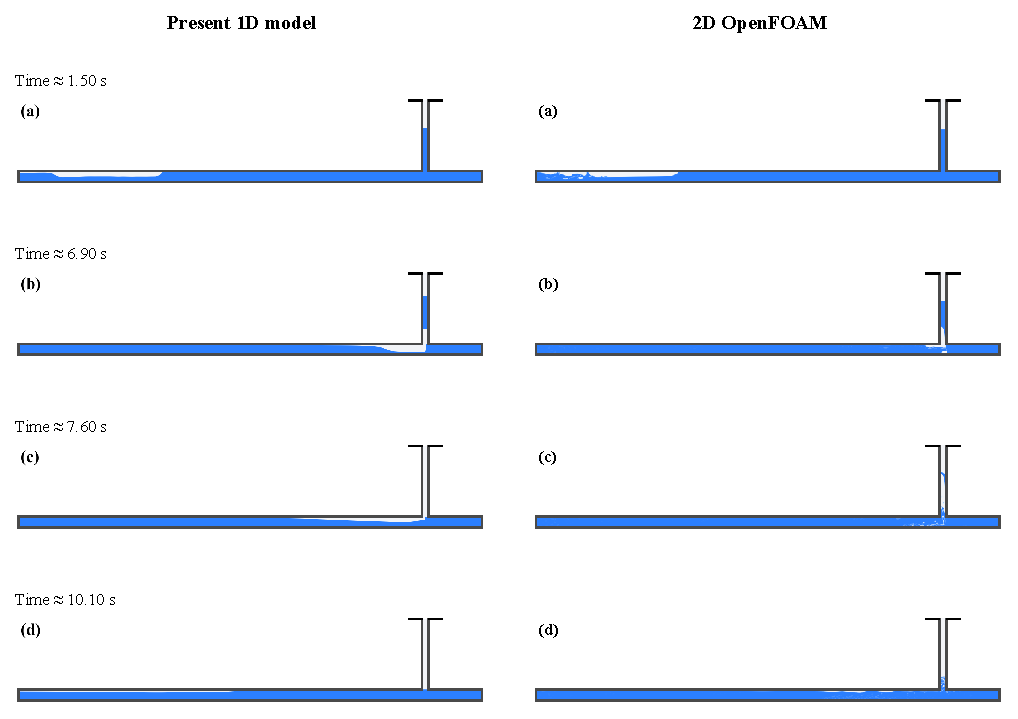
\includegraphics[width=\textwidth]{caseA_1d2d_snapshots_4frame.pdf}
\caption{Test~A phase evolution near $t=1.50$, $6.90$, $7.60$, and
$10.10$~s: present 1D model (left) and planar OpenFOAM simulation (right).
The corresponding archived 1D times are $1.480$, $6.908$, $7.608$, and
$10.108$~s, respectively; no time shift is applied. Blue denotes water and
white denotes gas. Row~(c) shows the breakthrough transition and rapid tower
drainage, and row~(d) shows the small residual-liquid region near the tower
base. In the 1D rendering only, cells with $\alpha_l\leq0.02$ are visually
omitted while their liquid volume remains in the equivalent-height audit.}
\label{fig:caseA_snapshots}
\end{figure}

The native-time histories in Fig.~\ref{fig:caseA_curves} provide the
quantitative comparison. The one-dimensional history is an explicitly
isolated sensitivity. It combines the contact-preserving release update with a
connected-pocket pressure-relaxation closure of time scale $\tau_b=0.10$~s.
This optional closure probes unresolved exchange between the coherent pocket
and the draining wall film, and it is not used for the other campaign claims.
The values below characterize the disclosed sensitivity rather than an
independently validated production closure.

The pre-venting pressure scale is close to the experiment, but the terminal
release remains late. Over
$4\leq T_{\mathrm{rel}}^{*}\leq7.5$, the one-dimensional plateau median is
$H^{*}=0.539$, compared with $0.537$ for the extracted experimental central
trace. After hydrostatic conversion from the probe elevation, the
crown-referenced two-dimensional mean is $0.562$ over
$1\leq T_{\mathrm{rel}}^{*}\leq7$. This datum conversion is not a fitted
offset. The main discrepancy lies in the release clock. The experimental,
two-dimensional, and one-dimensional traces first fall below $H^{*}=0.30$ at
$T_{\mathrm{rel}}^{*}=8.28$, 8.63, and 9.20, respectively. The
one-dimensional sensitivity therefore preserves the plateau but delays
terminal depressurization by about $0.92$ dimensionless time units. No time or
pressure shift is applied.

The short one-dimensional spike near $T_{\mathrm{rel}}^{*}=9.18$ coincides
with the archived level-coalescence event. It is retained for provenance but
is not interpreted as a resolved physical pressure rebound or included in the
plateau statistic.

All three records remain below the rim, and the one-dimensional level-event
times fall within the experimental spread.
The one-dimensional free surface rises gradually to
$Y^{*}_{fs,\max}=0.613$. The largest digitized
experimental marker is $0.649$, and the two-dimensional maximum is $0.623$;
none reaches the rim. The one-dimensional interface crosses
$Y^{*}_{int}=0.05$ at $T_{\mathrm{rel}}^{*}=7.85$. The raw archive reaches
exact equality with the free surface at 9.18, whereas the displayed trace stops
at the one-cell criterion at 9.13. Across the three digitized repetitions, the
first markers above the same $Y^{*}_{int}=0.05$ threshold span approximately
7.36--7.94. Piecewise-linear crossings of the digitized interface and
free-surface tracks span approximately 8.85--9.19. Both one-dimensional event
times lie within the observed run-to-run spread, although the sensitivity does
not reproduce the fastest interface rise. The sensitivity captures the
non-geysering outcome, pressure plateau, and maximum free-surface scale, but
terminal depressurization remains late. The remaining shape differences are
consistent with unresolved coherent-core/wall-film exchange. These data do not
identify that mechanism uniquely.

\begin{figure}[htbp]
\centering
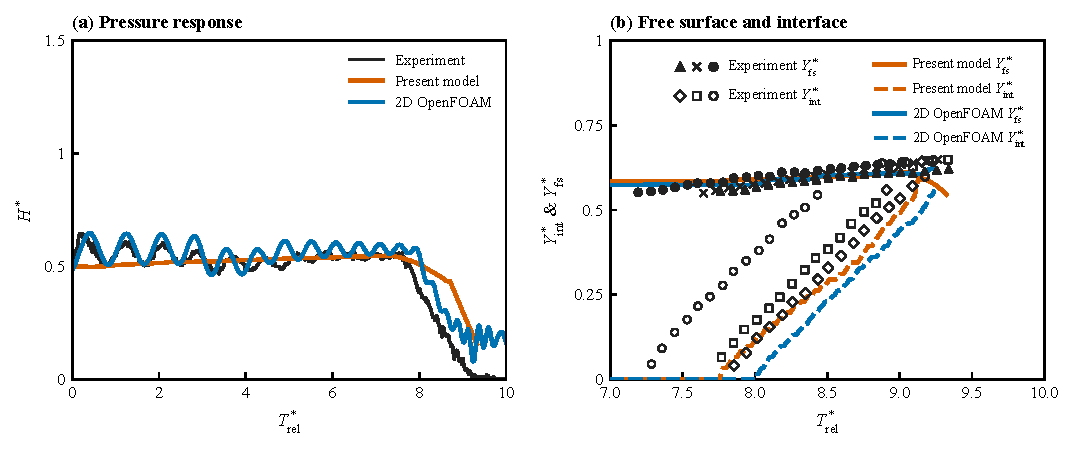
\includegraphics[width=\textwidth]{caseA_experiment_1d2d_curves.pdf}
\caption{Test~A comparison with \cite{vasconcelos2011}: (a) pressure head and
(b) normalized free-surface and interface elevations. Black denotes the
experiment, orange the present 1D model, and blue OpenFOAM.}
\label{fig:caseA_curves}
\end{figure}

The planar OpenFOAM calculation is a supporting spatial diagnostic rather than
a geometry-exact reference. In the vertical plane, the tower-to-pipe area
ratio is $D_t/D=0.607$. The circular apparatus instead has
$A_t/A_p=(D_t/D)^2=0.369$. The planar model also cannot reproduce a
three-dimensional annular wall film. Quantitative assessment is therefore
anchored to the experiment.
Within that scope, Test~A supports the wide-tower branch and the bulk pressure
and water-level scales, while revealing a systematic late bias in terminal
pocket depressurization. The interface event times remain within the digitized
three-run spread. This non-geysering reference provides the controlled contrast
for the narrow-tower Test~B; it is not an independent validation of the
optional connected-pocket closure.

\FloatBarrier

\subsubsection{Test B: small tower, geysering branch
($D_t/D=0.135$)}
\label{sec:tests:vw2011:caseB}

The narrow tower provides the geysering counterpart to Test~A. Vasconcelos and
Wright reported a geyser in every repetition. In the three Fig.~8 records, gas
first appears in the tower over $T_{\mathrm{rel}}^{*}=3.648$--$3.742$. The free
surface reaches the rim over $T_{\mathrm{rel}}^{*}=3.900$--$3.981$ and therefore
precedes gas breakthrough. The credible high-interface markers occur over
$T_{\mathrm{rel}}^{*}=4.09$--$4.17$. The Fig.~6 transducer record has a
pre-release plateau near $H^{*}=0.76$ and a collapse envelope of approximately
$T_{\mathrm{rel}}^{*}=4.02$--$4.18$ \cite{vasconcelos2011}.
The $D_t/D=0.135$ velocities in the source Table~2 are averages over the
tower-diameter group rather than measurements for this centre-panel condition,
so they are used only as contextual scales.  The source Fig.~11 is likewise
not imported: although it uses the same tower diameter, its initial head and
water level are $0.305$ and $0.254$~m, respectively, and therefore define a
different test.

The quantitative one-dimensional history uses a crown-datum pressure and a
pressure-driven tracked-front application closure. Its
Test~B mouth resistance and coverage
parameters were selected from a predeclared six-point bounded screen:
$K_{\mathrm{slug}}/K_{\mathrm{g}}=1.25$, 1.50, or 1.75, and
$\alpha_{g,\mathrm{j}}^{\mathrm{full}}=0.10$ or 0.12. The admissible 1.50/0.10
pair minimized the native interface error. The resulting errors are in-sample
closure diagnostics rather than an independent calibration test. No time
shift, curve fit, or level-trajectory smoothing is introduced.
The spatial snapshots serve a different role from the quantitative history.
Figure~\ref{fig:caseB_snapshots} uses a separate visualization archive. Its
horizontal state is Tosan-based, and its tower is reconstructed from saved
$Y_{fs}$, $Y_{int}$, and jet-height scalars. It supports morphological
comparison rather than quantitative tower-field validation. The planar
OpenFOAM calculation also serves only as an independent spatial diagnostic. It
retains the published pipe lengths and initial heads, but uses the
area-equivalent slit width $W=D_t^2/D$ and neglects surface tension. It is a
controlled two-dimensional surrogate for the release pathway, not a
geometry-exact representation of the $12.7$-mm circular tower.

The quantitative one-dimensional archive selects the observed geysering
branch. The standard two-dimensional archive selects the same branch. In the
one-dimensional result, the shock-fitted gas front crosses
$Y^{*}_{int}=0.05$ at $T_{\mathrm{rel}}^{*}=3.622$. The conservative
free-surface observer reaches the predeclared one-cell rim-completion level at
$T_{\mathrm{rel}}^{*}=3.923$, where $1-\Delta z/L=0.984$. This occurs before the
computed front/free-surface catch at $T_{\mathrm{rel}}^{*}=4.051$. The
corresponding two-dimensional entry and rim events occur at
$T_{\mathrm{rel}}^{*}=3.85$ and $4.11$. Both calculations therefore place rim
arrival ahead of the resolved upper-interface trajectory, although the
two-dimensional surrogate develops the sequence later. The archived
two-dimensional window does not resolve a subsequent gas-core catch, and none
is inferred from this comparison. The three rows in
Fig.~\ref{fig:caseB_snapshots} compare the complete pipe--tower domain at the
same physical times without event alignment: gas-pocket approach at
$t=6.35$~s, tower entry and water-column lift at $7.25$~s, and the initial
discharge/venting response at $7.70$~s. This common clock exposes the timing
difference; the rows do not supply the event metrics quoted above.

\begin{figure}[htbp]
\centering
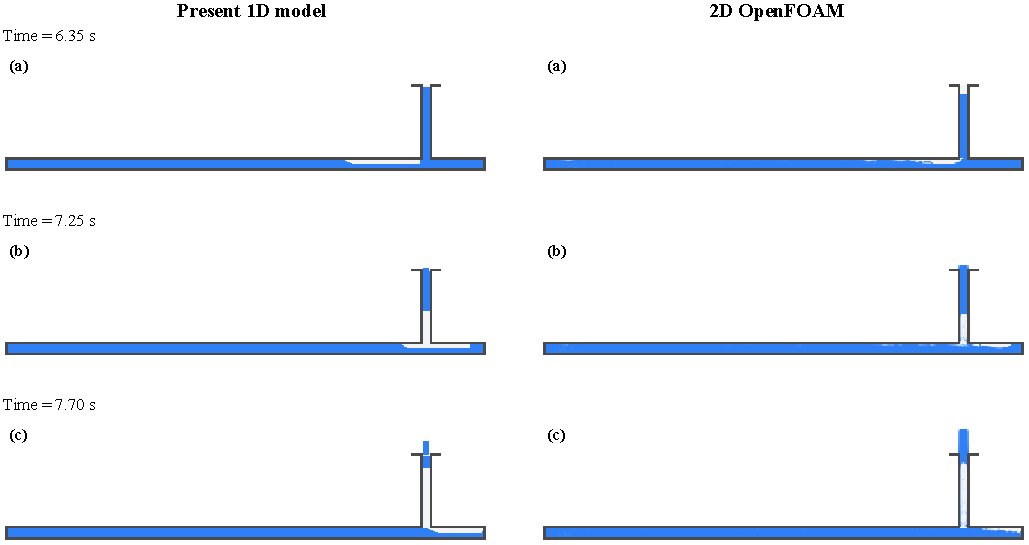
\includegraphics[width=\textwidth]{caseB_1d2d_snapshots_3frame_current.pdf}
\caption{Test~B phase evolution at $t=6.35$, $7.25$, and $7.70$~s:
present 1D model (left) and planar OpenFOAM simulation (right). Blue denotes
water and white denotes gas.}
\label{fig:caseB_snapshots}
\end{figure}

The native-time histories in Fig.~\ref{fig:caseB_curves} separate close
one-dimensional agreement in the bulk scales from larger event-timing and
two-dimensional biases. The experimental pre-eruption stand is
$Y^{*}_{fs}=0.823$, compared with $0.834$ in the one-dimensional model and
$0.869$ in the two-dimensional surrogate. At the crown datum, the
one-dimensional pressure plateau is $H^{*}=0.754$, versus the digitized
experimental pseudo-median value $0.758$ used in
Table~\ref{tab:caseB_summary}. The black curve itself is the pointwise
arithmetic mean of the three digitized repetitions. The standard raw
two-dimensional pre-release mean is higher, $H^{*}=0.838$ over
$1\le T_{\mathrm{rel}}^{*}\le3$. The displayed 0.40-s one-dimensional pressure
mean falls below $H^*=0.30$ at $T_{\mathrm{rel}}^{*}=4.097$, within the
experimental collapse envelope. The standard two-dimensional head crosses the
same threshold at $4.823$. All of these comparisons retain the native time
coordinate. For the shape-only comparison in
Fig.~\ref{fig:caseB_curves}(a), the blue pressure history comes from a separate
full-open-rim two-dimensional archive. It is displayed after one constant
offset, $\Delta H^{*}=-0.104$; no time shift or shape fit is applied. This
curve is excluded from the raw quantitative metrics. All quoted
two-dimensional pressure values and Table~\ref{tab:caseB_summary} use the
standard, unshifted-amplitude archive.

\begin{figure}[htbp]
\centering
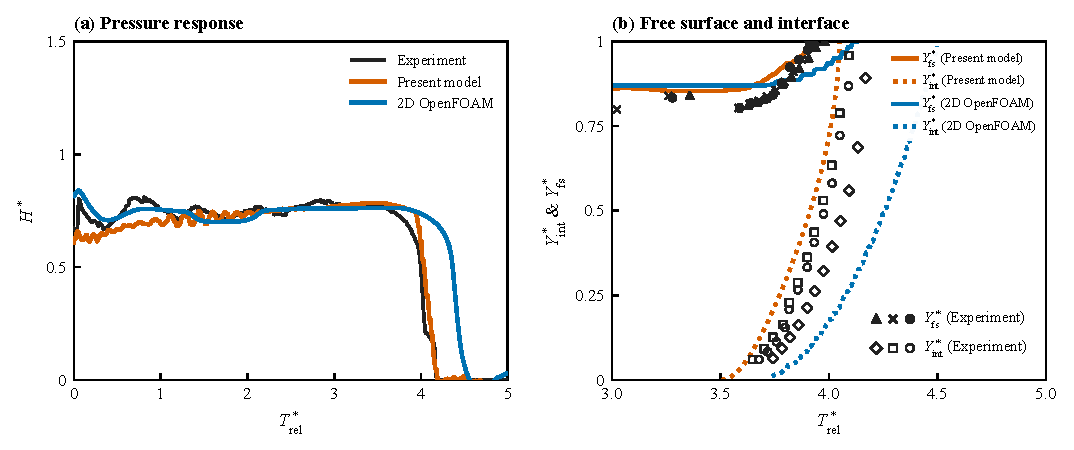
\includegraphics[width=\textwidth]{caseB_experiment_1d2d_curves.pdf}
\caption{Test~B comparison with \cite{vasconcelos2011}: (a) normalized
pressure head and (b) normalized free-surface and interface elevations.
Black denotes the experiment, orange the present 1D model, and blue OpenFOAM.}
\label{fig:caseB_curves}
\label{fig:caseB_pressure}
\label{fig:caseB_levels}
\end{figure}

The level histories recover the rising curvature, but the tracked interface
remains too early and high. The isolated digitized point at
$(T_{\mathrm{rel}}^{*},Y^{*})=(3.847,0.92)$ is retained in the plot for
provenance. It is not used as an arrival estimate because it lies
outside all three rising-interface tracks. Zero-level baseline/sentinel symbols
outside the rising tracks are also excluded from the trajectory comparison and
are not treated as positive-height measurements. With these symbols excluded,
the native-time rising-track RMSEs are $0.042$ and $0.206$ for the
one-dimensional $Y^{*}_{fs}$ and $Y^{*}_{int}$ histories, respectively; their
signed biases are $+0.034$ and $+0.172$. Both computed tracks accelerate over
the rising bands, with late-to-early slope ratios of 1.37 and 1.96. The
corresponding two-dimensional RMSEs remain $0.052$ and $0.303$. The revised
native curvature therefore removes the former piecewise-linear shape error,
but not the early, high interface bias. The connected cellwise
$\alpha_g=0.50$ field front reaches only $0.016L$ in this calculation.
Accordingly, $Y^{*}_{int}$ denotes the computed shock-fitted front closure
rather than a resolved dense-core isocontour. No plotting or digitization
offset is used to remove the remaining separation.

\FloatBarrier

\begin{table}[htbp]
\centering
\caption{Native-time, unshifted-amplitude Test~B validation summary.
Experimental intervals are
digitized three-run spans from the centre panels of Figs.~6 and~8 in
\cite{vasconcelos2011}; scalar experimental values use the digitized
pseudo-median, whereas the black pressure curve in
Fig.~\ref{fig:caseB_curves}(a) is the pointwise three-run mean. The 2D column
uses the standard raw archive and excludes the display-offset blue pressure
curve. The one-dimensional pressure-collapse row uses the same 0.40-s
centered mean shown in panel (a); its level-event rows use native samples.}
\label{tab:caseB_summary}
\begin{tabular}{lccc}
\toprule
Observable & Experiment & 1D & 2D \\
\midrule
Outcome & geyser, 3/3 & geyser & geyser \\
Pre-release $H^{*}$ & 0.758 & 0.754 & 0.838 \\
Pre-entry $Y^{*}_{fs}$ & 0.823 & 0.834 & 0.869 \\
$Y^{*}_{int}=0.05$ crossing, $T_{\mathrm{rel}}^{*}$ & 3.648--3.742 & 3.622 & 3.848 \\
First rim arrival, $T_{\mathrm{rel}}^{*}$ & 3.900--3.981 & 3.923$^{\mathrm{a}}$ & 4.114 \\
Pressure pseudo-median $H^{*}<0.30$, $T_{\mathrm{rel}}^{*}$ & 4.048 & 4.097 & 4.823 \\
\bottomrule
\end{tabular}
\vspace{0.3em}

\parbox{0.98\linewidth}{\footnotesize $^{\mathrm{a}}$The one-dimensional
rim event uses the predeclared one-cell completion criterion
$Y^{*}_{fs}\ge 1-\Delta z/L=0.9836$; the topology latch and plotted
geometric observer cross it at the same native sample.}
\end{table}

Table~\ref{tab:caseB_summary} reports only quantities that can be compared
without differentiating sparse video markers. The scalar experimental
pressure values are read from the digitized pseudo-median; the reported event
intervals retain the visible three-run scatter. Both calculations reproduce
the outcome and event ordering. Relative to the experimental intervals, the
one-dimensional tracked front begins slightly early and remains too high, but
the grid-complete rim event and pressure collapse fall within the measured
spans. The two-dimensional surrogate enters slightly late, spills late, and
retains its excess head longest.

\FloatBarrier

Across the two tests, the archived branch evidence selects venting without
overflow in the wide tower and eruption in the narrow tower. The Test~A
connected-pocket sensitivity recovers the pressure and free-surface scales but
delays terminal depressurization; its interface event times remain within the
three-run spread. It is not conflated with the
separate spatial reconstruction. For Test~B, the quantitative one-dimensional
history closely reproduces the pre-eruption pressure and water-column scales,
while the shock-fitted interface remains early and high. The grid-complete
rim event and pressure collapse lie within the experimental spans.
The standard planar calculation supports the same entry-to-overflow morphology,
but overpredicts the pre-release head and water level and delays the principal
events. Quantitative comparison remains anchored to the experiment. The
two-dimensional results and display reconstructions provide supporting evidence
subject to the limitations stated in their captions. Section~\ref{sec:discussion}
relates the remaining timing pattern to the shaft-mouth and entrainment
closures.

\FloatBarrier

\subsection{Campaign 2: entrapped-air release from a horizontal pipe into a
vertical riser (Cong, Chan and Lee, 2017)}
\label{sec:tests:cong2017}

The apparatus of \cite{cong2017} consists of a horizontal acrylic pipe with
diameter $D=0.05$~m and length approximately $6$~m. Its upstream end is
connected to a constant-head tank, and a tee-junction supports a vertical riser
of height $1.8$~m and variable diameter ($D_r=16$--$46$~mm). An air pocket of
prescribed initial length $L_0$ is created in the horizontal pipe between ball
valves. Release under the upstream head $H_0$ drives the pocket along the pipe
crown to the riser, where it vents through the initially water-filled column.
Video and high-speed cameras recorded the air--water interface trajectories in
the pipe and riser. Transducers measured pressure near the pipe end and at the
riser base (Fig.~\ref{fig:cong_apparatus}).

\begin{figure}[htbp]
\centering
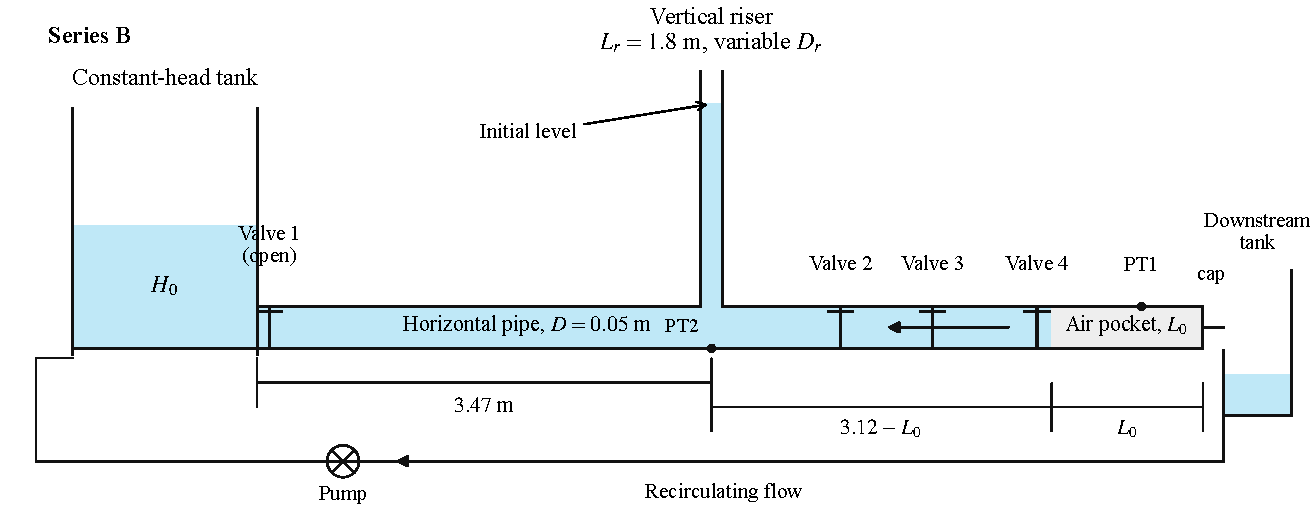
\includegraphics[width=\textwidth]{campaign2_apparatus_redrawn.pdf}
\caption{Campaign 2 Series-B apparatus, redrawn from Fig.~1(b) of
\cite{cong2017}.}
\label{fig:cong_apparatus}
\end{figure}

The authors summarized the outcomes of their parameter study with
a two-parameter geysering criterion,
\begin{equation}
\frac{D_r}{D}\le 0.62
\qquad\text{and}\qquad
V^{*}_{air}=\frac{V_{air}}{(\pi D_r^2/4)\,H_0}\ge 3.42,
\label{eq:cong_criterion}
\end{equation}
which requires both a sufficiently narrow riser and a pocket volume large
relative to the riser water column.

This campaign evaluates the model as a regime classifier over a systematic
sweep, rather than against individual time histories as in Campaign~1. The
first comparison treats the seven high-speed-camera runs of the experimental
Series~B individually (B-H1\,--\,B-H7: $H_0=0.66$~m, $L_0=0.61$~m, riser
diameters $D_r/D=0.32$--$0.92$). Computed classification, pocket arrival time,
and mean rise velocity are compared with the measurements. The second
comparison covers a broader synthetic sweep over the experimental parameter
ranges ($D_r=16$--$46$~mm, $L_0=0.61$--$1.8$~m,
$H_0=0.66$--$0.88$~m; 63 configurations). The resulting classifications are
compared with the experimental criterion in Eq.~(\ref{eq:cong_criterion}).

All campaign runs use the same fully synchronous junction coupling as
Campaign~1 and the identical frozen solver configuration (the Campaign~1
Test~B closure set). No parameter is changed between campaigns or between
runs. Two geometric features are specific to this apparatus. The upstream
boundary is the constant-head tank, and the pocket is created
\emph{downstream} of the riser tee. The released pocket therefore travels
upstream along the crown toward the riser. The tee position, 2.88~m from the
tank, is fixed from the experiment's kinematics. The measured arrival times
and front speeds in Table~2 of \cite{cong2017} give a valve-to-tee distance
$T_a\,U_f$ of $2.51$/$1.92$/$1.32$~m for the three pocket lengths
$L_0=0.61$/$1.2$/$1.8$~m, all placing the tee at the same station. This
position is held fixed across the sweep. An earlier campaign version used a
staged horizontal/vertical treatment whose classifier reduced to a static
volume--diameter criterion. Those results were circular as a validation of
Eq.~(\ref{eq:cong_criterion}) and are superseded by the fully coupled results
reported here.

\subsubsection{Series B: classification, arrival times, and rise velocities}
\label{sec:tests:cong2017:seriesB}

The model reproduces five of the seven measured Series-B classifications
(Table~\ref{tab:cong_bh} and Fig.~\ref{fig:cong_bh}). It predicts geysering for
B-H1 ($D_r/D=0.32$) and no geysering for B-H4--B-H7
($D_r/D=0.62$--$0.92$), with no false positives. The two intermediate
geysering runs, B-H2 and B-H3 ($D_r/D=0.42$, $0.52$), are misclassified as
non-geysering. Their computed free surfaces rise to $0.87$ and $0.82$~m but do
not reach the rim. The error is one-sided: the model under-predicts eruption.
Section~\ref{sec:discussion} examines how volume-neutral mouth exchange may
contribute to this bias. The same exchange allows the narrow-riser pocket to
rebuild the overpressure that powers the B-H1 geyser, but it also cancels part
of the one-to-one column lift in the reservoir-fed layout as riser width
increases. The computed arrival times are late by $1.5$~s on average, with the
largest delay in the widest riser where the arrested crown current covers the
final reach slowly. The measured spread is $7.84$--$8.22$~s.

The rise-speed comparison reveals an overly pulsed computed response. In the
geysering run B-H1, the computed eruption-window climb speeds
($v_{fs}=1.71$, $v_{int}=1.28$~m/s as the fastest sustained $0.6$-s climb)
exceed the respective measured whole-event means ($0.92$, $1.23$~m/s). The
interface speed is close, but the free-surface speed is markedly high. The
eruption jet is therefore over-sharp, consistent with the narrow-riser bias
found in Test~B of Campaign~1. In the no-geysering branch, the computed gas-nose climb speeds
($0.69$--$1.20$~m/s) exceed the measured $0.42$--$0.48$~m/s. The computed
climb is concentrated in surge pulses rather than the observed steady
Taylor-scale ascent. The computed free-surface response
($0.20$--$0.65$~m/s during the pulses, zero sustained rise) has the same pulsed
character, compared with the measured steady $0.2$--$0.26$~m/s.

The synchronous coupling recovers the measured ranking of the pipe-end
pressure transients. The geysering run B-H1 develops a cycle-averaged
compression surge to $1.71\,H_0$, compared with the reported value of about
$1.9\,H_0$. The no-geysering run B-H6 shows only a gentle post-arrival hump to
$1.02\,H_0$, compared with the reported value of about $1.4\,H_0$. The staged
treatment gave both runs the same $2.07\,H_0$ peak. The synchronous coupling
instead recovers the experimental differentiation: a wide riser vents the
pocket and thereby damps the pipe-end pressure. This gain is accompanied by
the two intermediate-diameter classification misses discussed above.

\begin{table}[htbp]
\centering
\caption{Campaign 2, experimental Series B of \cite{cong2017}
($H_0=0.66$~m, $L_0=0.61$~m): measured against computed classification,
pocket arrival time $T_a$, maximum computed free-surface height
$Y_{fs,\max}$ (riser top at $1.8$~m), and rise speeds of the free surface
($v_{fs}$) and gas nose ($v_{int}$). Measured speeds are whole-event means
(Table~2 of \cite{cong2017}); computed speeds are the fastest sustained
$0.6$-s climb in the venting window. Misclassified runs are marked
$^{\dagger}$.}
\label{tab:cong_bh}
\resizebox{\textwidth}{!}{%
\begin{tabular}{lcccccccccc}
\toprule
& & & \multicolumn{2}{c}{Geysering} & \multicolumn{2}{c}{$T_a$ (s)}
& & \multicolumn{2}{c}{$v_{fs}$ (m/s)} & $v_{int}$ (m/s) \\
\cmidrule(lr){4-5}\cmidrule(lr){6-7}\cmidrule(lr){9-10}
Run & $D_r/D$ & $V^{*}_{air}$ & Meas. & Model & Meas. & Model
& $Y_{fs,\max}$ (m) & Meas. & Model & Meas. / Model \\
\midrule
B-H1 & 0.32 & 9.03 & yes & yes & 8.07 & 7.56 & 1.80 & 0.92 & 1.71 & 1.23 / 1.28 \\
B-H2$^{\dagger}$ & 0.42 & 5.24 & yes & no & 7.84 & --   & 0.87 & 0.77 & --   & 1.02 / -- \\
B-H3$^{\dagger}$ & 0.52 & 3.42 & yes & no & 8.18 & 9.56 & 0.82 & 0.66 & 0.43 & 0.92 / 1.24 \\
B-H4 & 0.62 & 2.40 & no & no & 8.14 & 9.40  & 0.82 & 0.21 & 0.53 & 0.42 / 1.20 \\
B-H5 & 0.72 & 1.78 & no & no & 8.10 & 9.88  & 0.86 & 0.26 & 0.65 & 0.48 / 1.05 \\
B-H6 & 0.82 & 1.37 & no & no & 8.10 & 9.16  & 0.78 & 0.25 & 0.39 & 0.48 / 1.05 \\
B-H7 & 0.92 & 1.09 & no & no & 8.22 & 11.44 & 0.79 & 0.20 & 0.20 & 0.44 / 0.69 \\
\bottomrule
\end{tabular}
}
\end{table}

\begin{figure}[htbp]
\centering
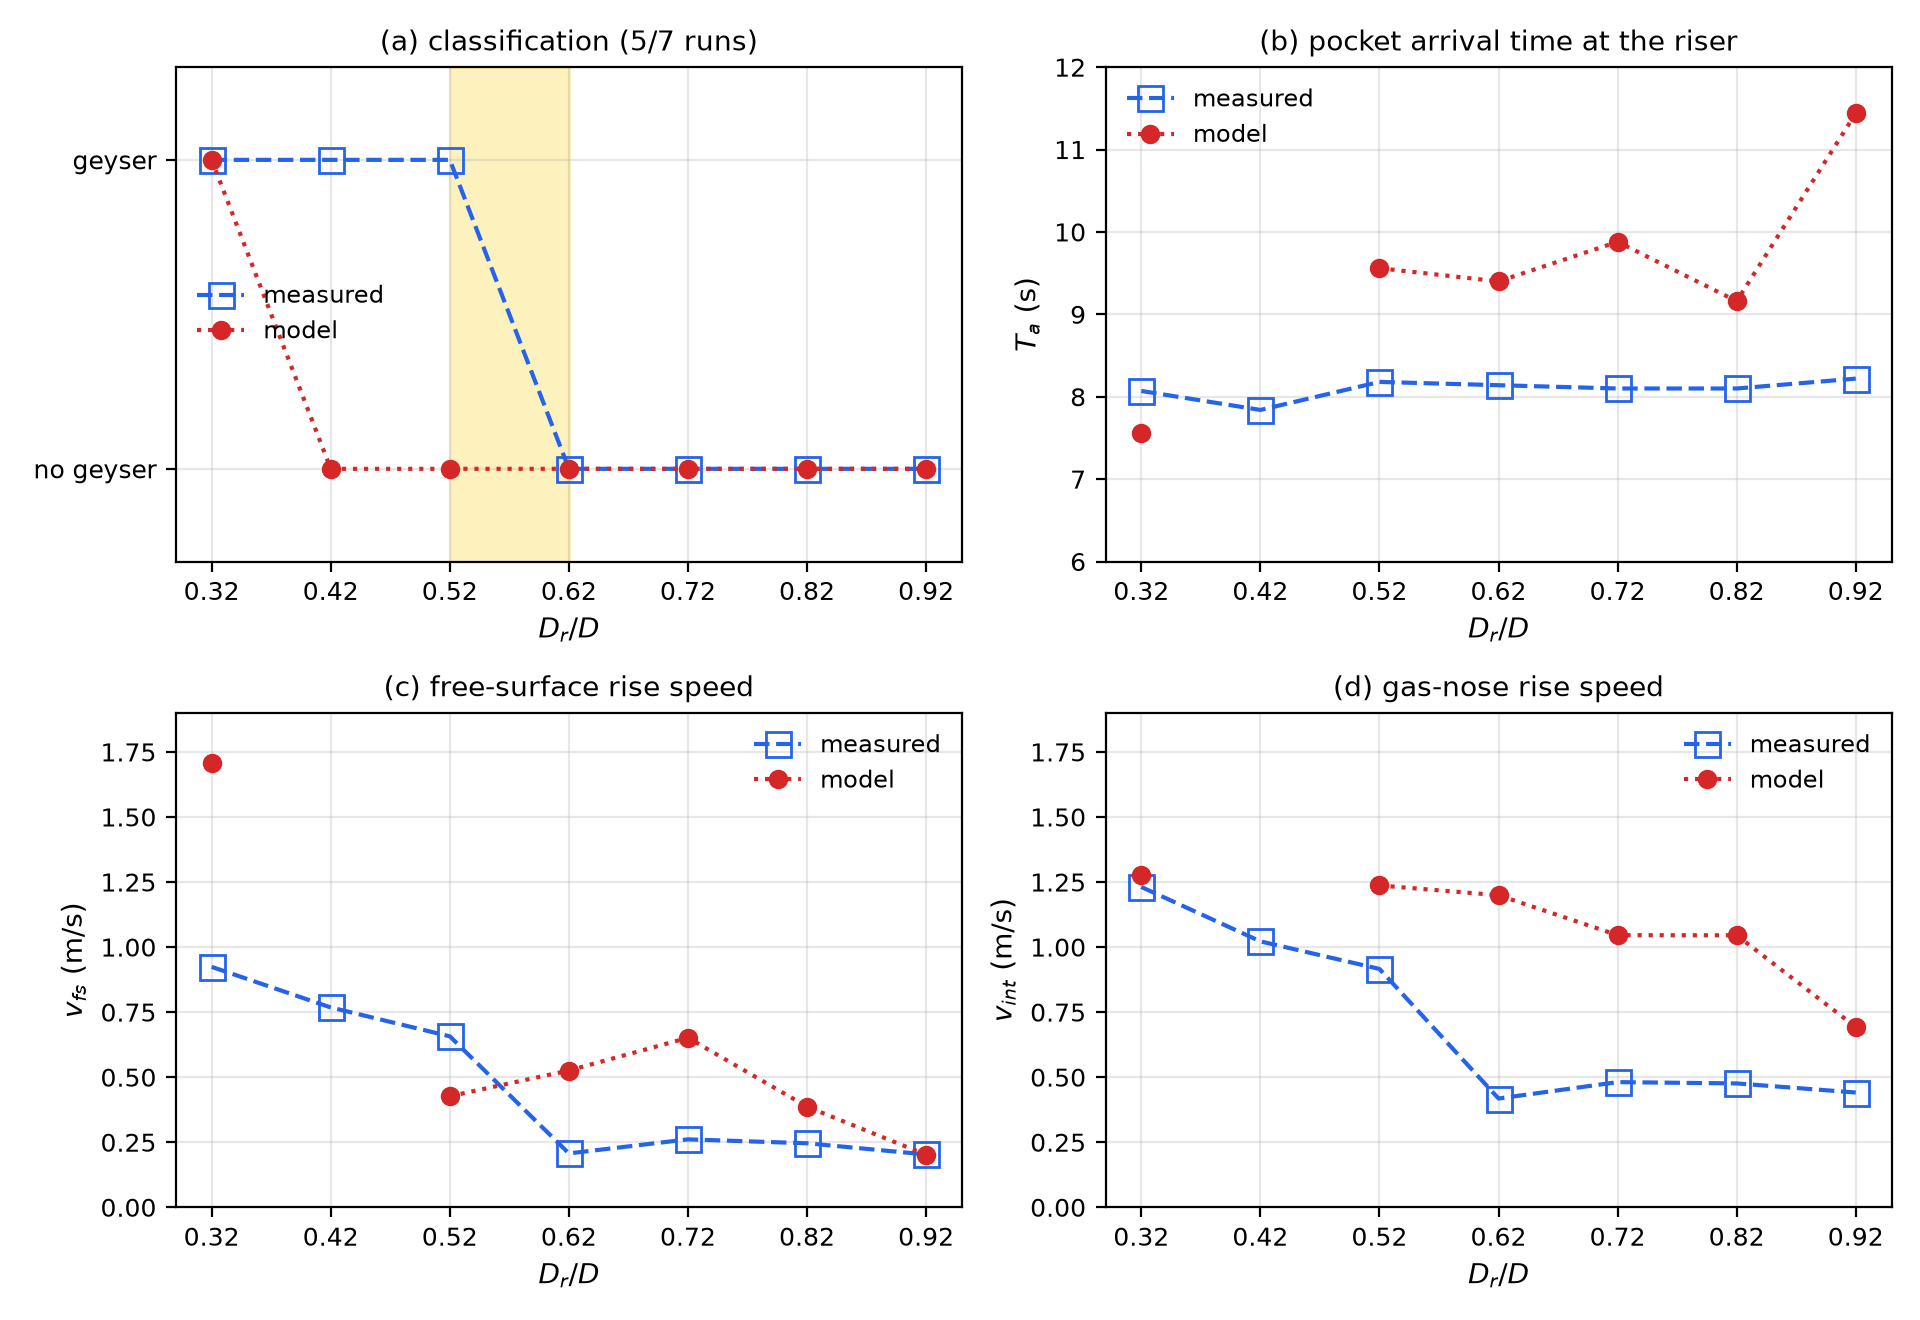
\includegraphics[width=\textwidth]{cong2017_bh_series.png}
\caption{Campaign 2 Series B \cite{cong2017}: (a) geysering classification,
(b) pocket-arrival time, (c) free-surface rise speed, and (d) gas-nose rise
speed versus $D_r/D$.}
\label{fig:cong_bh}
\end{figure}

The two signature runs clarify how riser diameter changes the pressure and
water-column response (Fig.~\ref{fig:cong_signature}). These runs are also
examined as individual histories in
Sections~\ref{sec:tests:cong2017:seriesB} and the case folders. Their archived
reproductions include per-run comparisons with the digitized level and pressure
histories from Figs.~7, 9 and~10 of \cite{cong2017}. In B-H1
($D_r/D=0.32$), the released pocket arrives at $7.56$~s (measured $8.07$~s).
The entering gas drives the free surface upward in two surge pulses, while
arrest of the supply-line counter-flow compresses the pocket to
$1.71\,H_0$ (cycle-averaged; reported $\approx1.9\,H_0$). The resulting column
ejection places the free surface at the rim while the gas nose remains below
it, which is the geysering signature. In B-H6 ($D_r/D=0.82$), the same release
delivers the same pocket, but the wide riser passes the gas with only a gentle
free-surface rise to $0.78$~m. The pocket vents without eruption, and its
pressure never exceeds $1.02\,H_0$ after arrival. Because only $D_r$ changes,
the pipe-end pressure provides the experiment's cleanest controlled contrast.
The model reproduces its sign and ranking, although both pressure levels are
under-predicted. The $1.4\,H_0$ no-geyser hump is missed because the computed
free-surface lift is under-predicted in the reservoir-fed layout
(Section~\ref{sec:discussion}).

\begin{figure}[htbp]
\centering
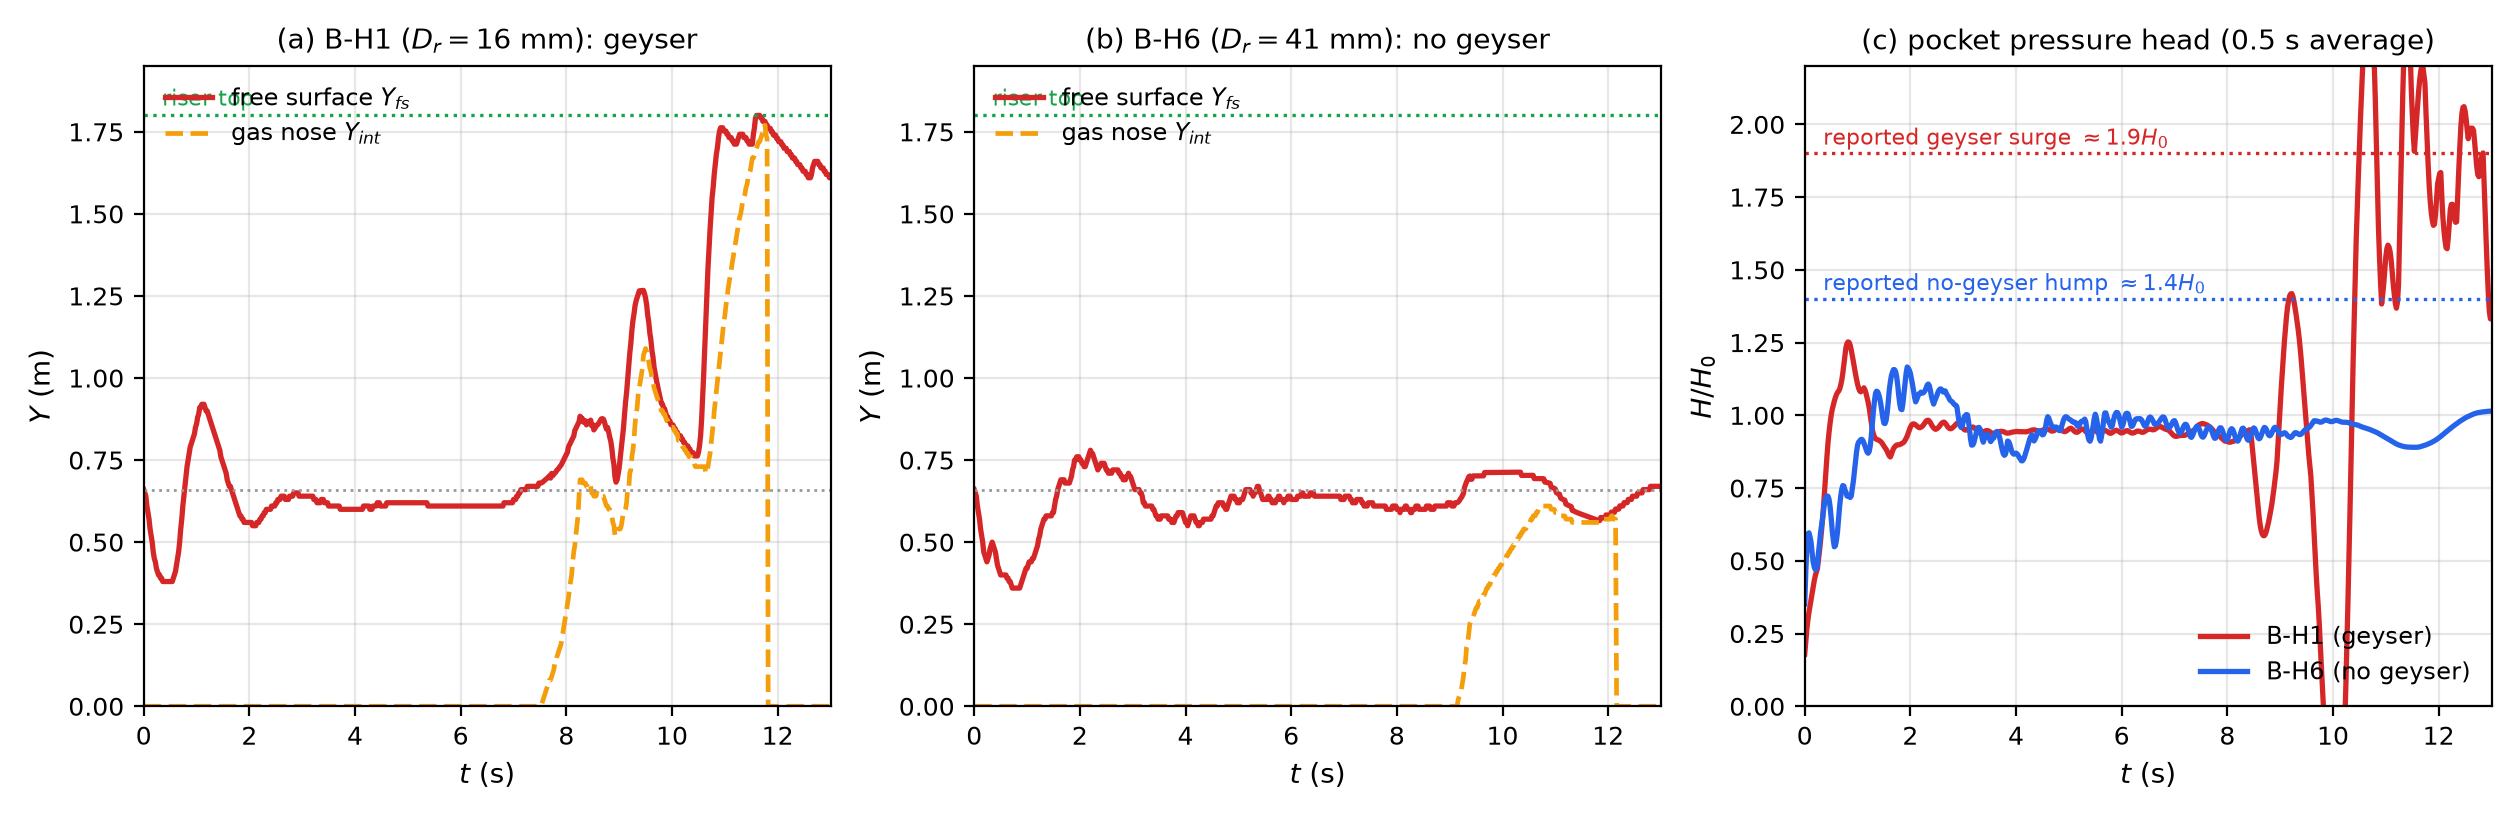
\includegraphics[width=\textwidth]{cong2017_signature.png}
\caption{Campaign 2 signature cases \cite{cong2017}: free-surface and gas-nose
trajectories for (a) B-H1 and (b) B-H6, and (c) their pocket-pressure heads.}
\label{fig:cong_signature}
\end{figure}

The common-clock spatial comparison for B-H1 supports the same branch but
exposes different eruption clocks (Fig.~\ref{fig:cong_bh1_1d2d}). At the
physical times $8.5$, $12.8$, and $13.0$~s, the frozen 1D archive reports a
much earlier free-surface rise. It reaches $1.79$~m above the pipe crown by
$13.0$~s, whereas the refined planar OpenFOAM field still places the water
column below the $1.8$~m rim. The 2D calculation reaches $98\%$ of the rim at
$13.865$~s and resolves water above $2.1$~m at $14.8$~s. Both descriptions
select the measured geysering branch, but their eruption clocks and spatial
representations differ. The 2D gas-arrival time, $8.50$~s, is close to the
measured $8.07$~s. Its subsequent eruption is nevertheless late relative to
the reported $9.55$~s, and its post-arrival pressure surge is not reproduced.
The sequence therefore provides supporting evidence for branch selection and
morphology, not a quantitative OpenFOAM validation.

\begin{figure}[htbp]
\centering
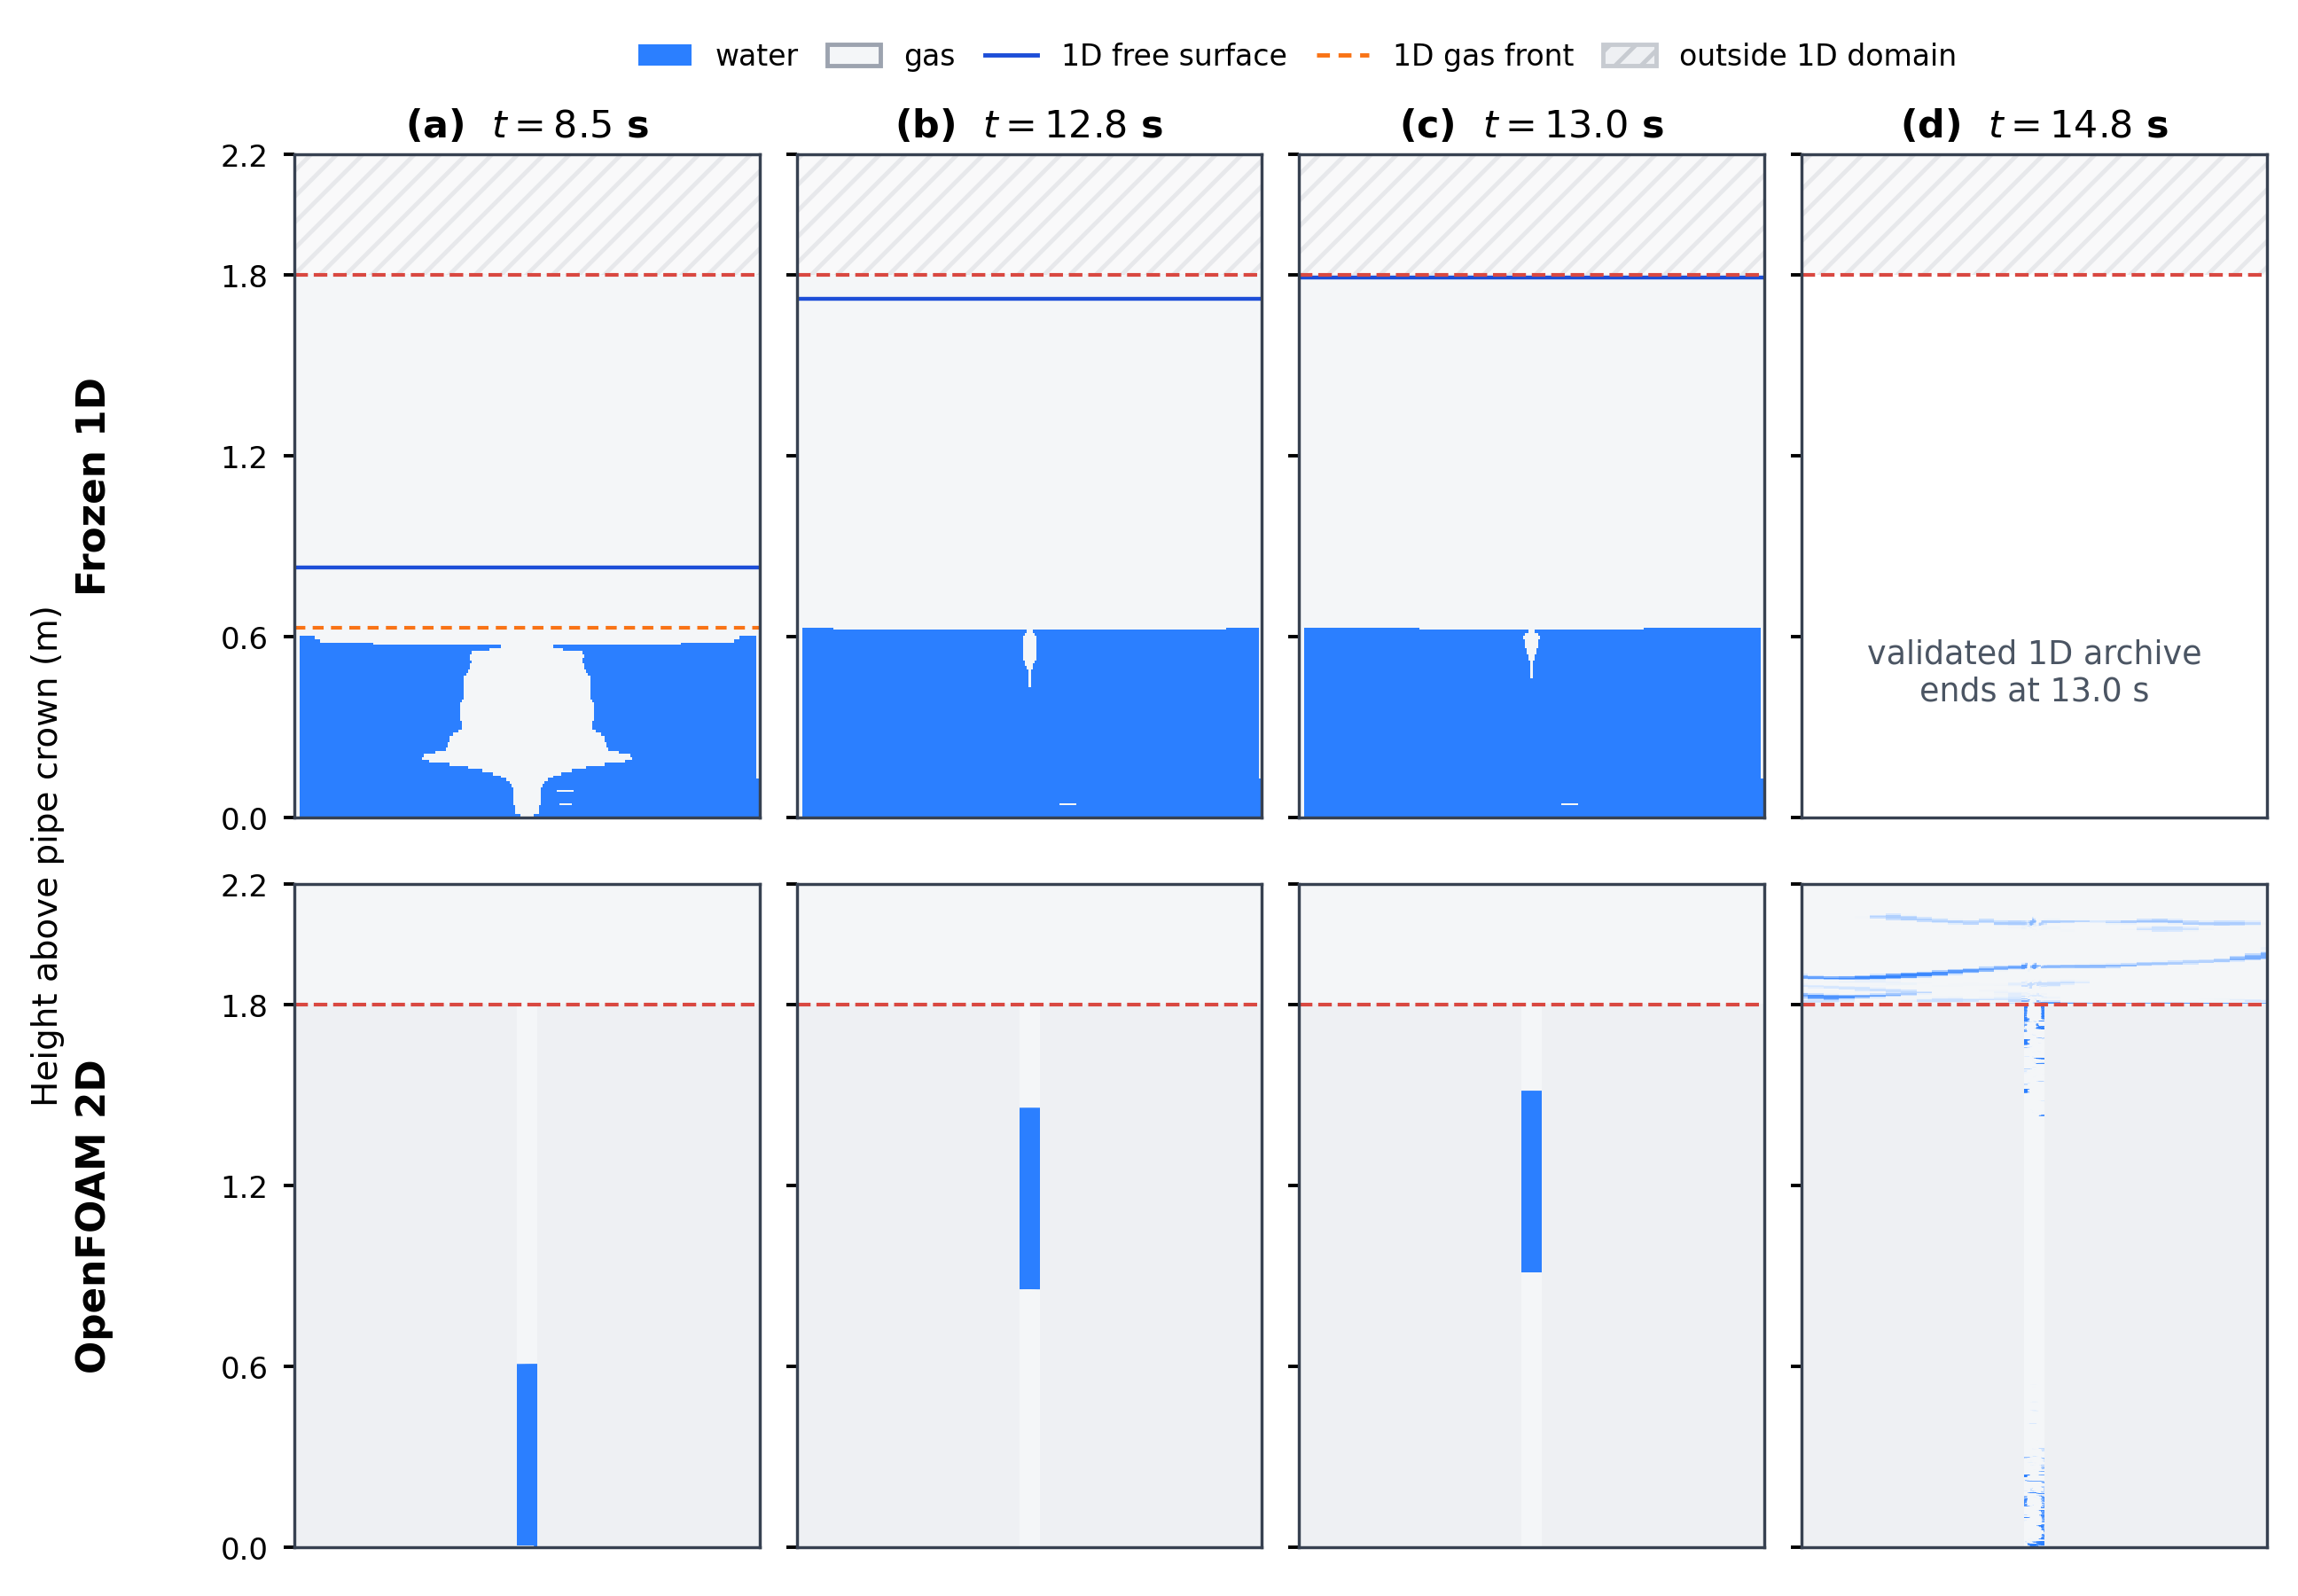
\includegraphics[width=\textwidth]{cong2017_bh1_1d2d_phase_sequence.png}
\caption{B-H1 riser phase sequence at $t=8.5$, $12.8$, $13.0$, and
$14.8$~s: present 1D model (top) and planar OpenFOAM simulation (bottom).
The archived 1D run ends at $13.0$~s.}
\label{fig:cong_bh1_1d2d}
\end{figure}

The complete-domain comparison for B-H6 preserves the observed non-geysering
sequence at the photographic clock (Fig.~\ref{fig:cong_bh6_multiframe}). The
three times correspond to gas arrival ($8.7$~s), developed rise ($9.9$~s), and
late venting ($10.9$~s). Each row places the published B-H6 riser photograph
between the full 1D and planar OpenFOAM domains, with no event alignment. The
1D reconstruction passes a compact gas pocket with weaker water-column lift,
whereas the 2D VOF field gives a stronger and more spatially distributed late
response. Because the high-speed record images the riser rather than the full
horizontal pipe, the photographic column validates the riser sequence. The
outer panels show the corresponding system-level phase distribution.

\begin{figure}[htbp]
\centering
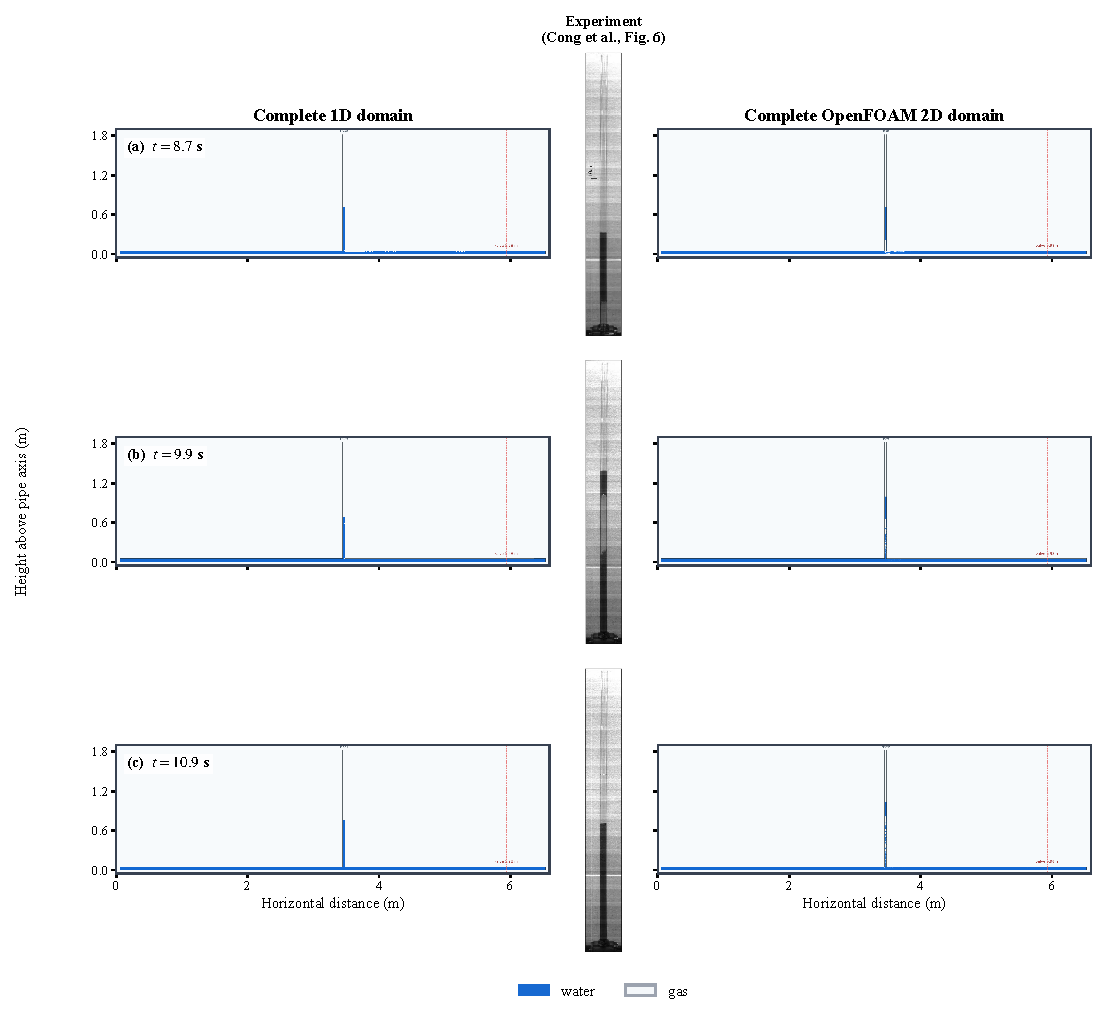
\includegraphics[width=0.98\textwidth]{cong2017_bh6_experiment_1d2d_full_domain_3frame.pdf}
\caption{B-H6 full-domain comparison at (a) $8.7$, (b) $9.9$, and
(c) $10.9$~s: present 1D model (left), experiment \cite{cong2017} (centre),
and planar OpenFOAM simulation (right).}
\label{fig:cong_bh6_multiframe}
\end{figure}

The aggregate Series-B comparison conceals how the two descriptions differ
within an individual non-geysering event. Figure~\ref{fig:cong_bh6_1d2d}
therefore overlays the digitized B-H6 markers from Fig.~7(a) of
\cite{cong2017} with a geometry-matched one-dimensional application and the
area-equivalent planar OpenFOAM calculation. All traces retain physical time;
only the dense two-dimensional trace receives a centred $0.05$-s running
median for display. Both calculations reproduce the observed non-geysering
outcome. The two-dimensional gas reaches the riser at $8.04$~s, close to the
measured $8.10$~s, whereas the one-dimensional arrival is $8.66$~s. The
trajectory comparison is less complete: free-surface marker RMSE is
$0.097$~m for the two-dimensional result and $0.310$~m for the
one-dimensional result, while gas-nose RMSE is $0.245$ and $0.317$~m,
respectively. Both under-predict the final lift, but the spatial calculation
substantially reduces the free-surface error.

The focused one-dimensional trace is a geometry- and valve-matched application
variant whose horizontal gas front uses the Benjamin-celerity closure; it is
shown to diagnose this case and does not replace the frozen Series-B values in
Table~\ref{tab:cong_bh}. Likewise, the planar calculation is supporting
evidence for spatial consistency rather than an expansion of the primary
validation scope.

\begin{figure}[htbp]
\centering
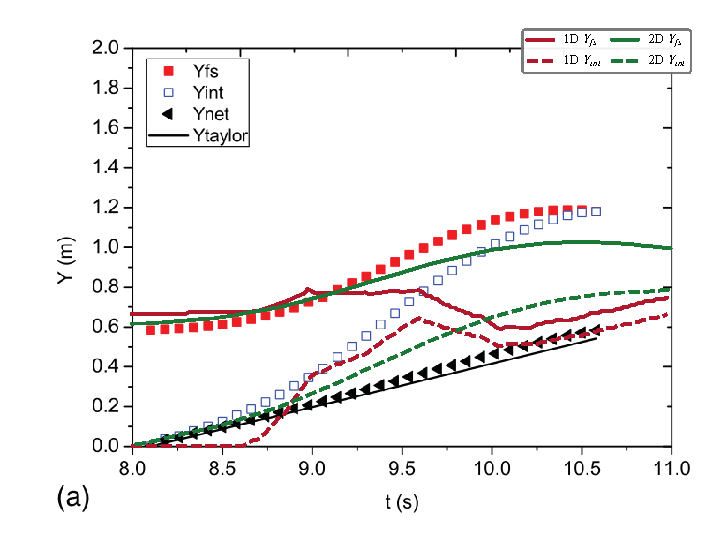
\includegraphics[width=\textwidth]{cong2017_fig7a_bh6_experiment_1d2d.pdf}
\caption{B-H6 free-surface ($Y_{fs}$, solid) and interface ($Y_{int}$,
dashed) trajectories overlaid on Fig.~7(a) of \cite{cong2017}. Dark red and
green denote the present 1D model and OpenFOAM, respectively.}
\label{fig:cong_bh6_1d2d}
\end{figure}

A source-matched comparison preserves the experimental parameter context by
transcribing the B-H6 row of Table~2 in \cite{cong2017}
(Table~\ref{tab:cong_bh6_source_matched}). The second block reports only
quantities available robustly from all three records. This makes the outcome
and arrival-time comparison explicit without substituting peak-based
simulation values for the source table's whole-event velocity definitions.

\begin{table}[htbp]
\centering
\caption{Source-matched B-H6 parameter and result comparison. The first block
transcribes the B-H6 row of Table~2 in \cite{cong2017}; the second block adds
the experimental, 1D, and OpenFOAM 2D outcome, gas-arrival time, peak levels,
and marker RMSE. Dashes denote quantities not defined for the experimental
reference.}
\label{tab:cong_bh6_source_matched}
\small
\begin{tabular}{@{}lclc@{}}
\toprule
\multicolumn{4}{c}{Published B-H6 condition and whole-event measures} \\
\midrule
Parameter & Value & Parameter & Value \\
\midrule
$D_r$ (m) & 0.041 & $H_0$ (m) & 0.66 \\
$L_0$ (m) & 0.61 & $T_a$ (s) & 8.10 \\
$U_f/\sqrt{gD}$ & 0.443 & $D_r/D$ & 0.82 \\
$V_{\mathrm{air}}/V_w$ & 1.37 & Geyser & No \\
$\overline{v}_{fs}$ (m/s) & 0.246 & $\overline{v}_{int}$ (m/s) & 0.476 \\
$\overline{v}_{net}$ (m/s) & 0.235 & $v_{\mathrm{Taylor}}$ (m/s) & 0.219 \\
\bottomrule
\end{tabular}

\vspace{0.7em}

\begingroup
\footnotesize
\setlength{\tabcolsep}{2.5pt}
\begin{tabular}{@{}lcccccc@{}}
\toprule
Source & Outcome & $T_a$ (s) &
\shortstack{$Y_{fs,\max}$\\(m)} &
\shortstack{$Y_{int,\max}$\\(m)} &
\shortstack{RMSE $Y_{fs}$\\(m)} &
\shortstack{RMSE $Y_{int}$\\(m)} \\
\midrule
B-H6 experiment & No & 8.10 & 1.201 & 1.178 & -- & -- \\
1D & No & 8.66 & 0.786 & 0.700 & 0.310 & 0.317 \\
OpenFOAM 2D & No & 8.04 & 1.021 & 0.940 & 0.097 & 0.245 \\
\bottomrule
\end{tabular}
\endgroup
\end{table}

\FloatBarrier

\subsubsection{Regime map against the experimental criterion}
\label{sec:tests:cong2017:map}

The 63-configuration sweep yields a one-sided missed-eruption bias in the
criterion plane $(D_r/D,\ V^{*}_{air})$
(Fig.~\ref{fig:cong_map}). Each point represents one full synchronous
simulation classified without knowledge of Eq.~(\ref{eq:cong_criterion}); the
criterion lines are drawn only for comparison. The model agrees with the
experimental criterion in 39 of 63 configurations. In all 24 disagreements,
the criterion predicts geysering and the model does not. There are no false
positives. Every modelled eruption lies inside the criterion's geysering
region. The no-geysering half-plane $D_r/D>0.62$ and the small-volume region
$V^{*}_{air}<3.42$ are classified correctly throughout. The misses concentrate
at intermediate diameters ($D_r/D=0.42$--$0.62$) combined with large pocket
volumes ($L_0\ge1.2$~m). In these cases, the computed free surface rises to
$1.0$--$1.6$~m but remains below the $1.8$-m rim; seven of the 24 reach within
$0.45$~m of it. This pattern extends the Series-B under-lift bias across the
parameter plane. The model retains both end members and the interaction that
eruption requires narrow risers \emph{and} large relative pocket volume, but
requires more restrictive conditions for eruption and under-predicts it in the
transition band. For screening, the bias direction is consequential: the
frozen model misses geysers near the boundary rather than producing false
alarms.

\begin{figure}[htbp]
\centering
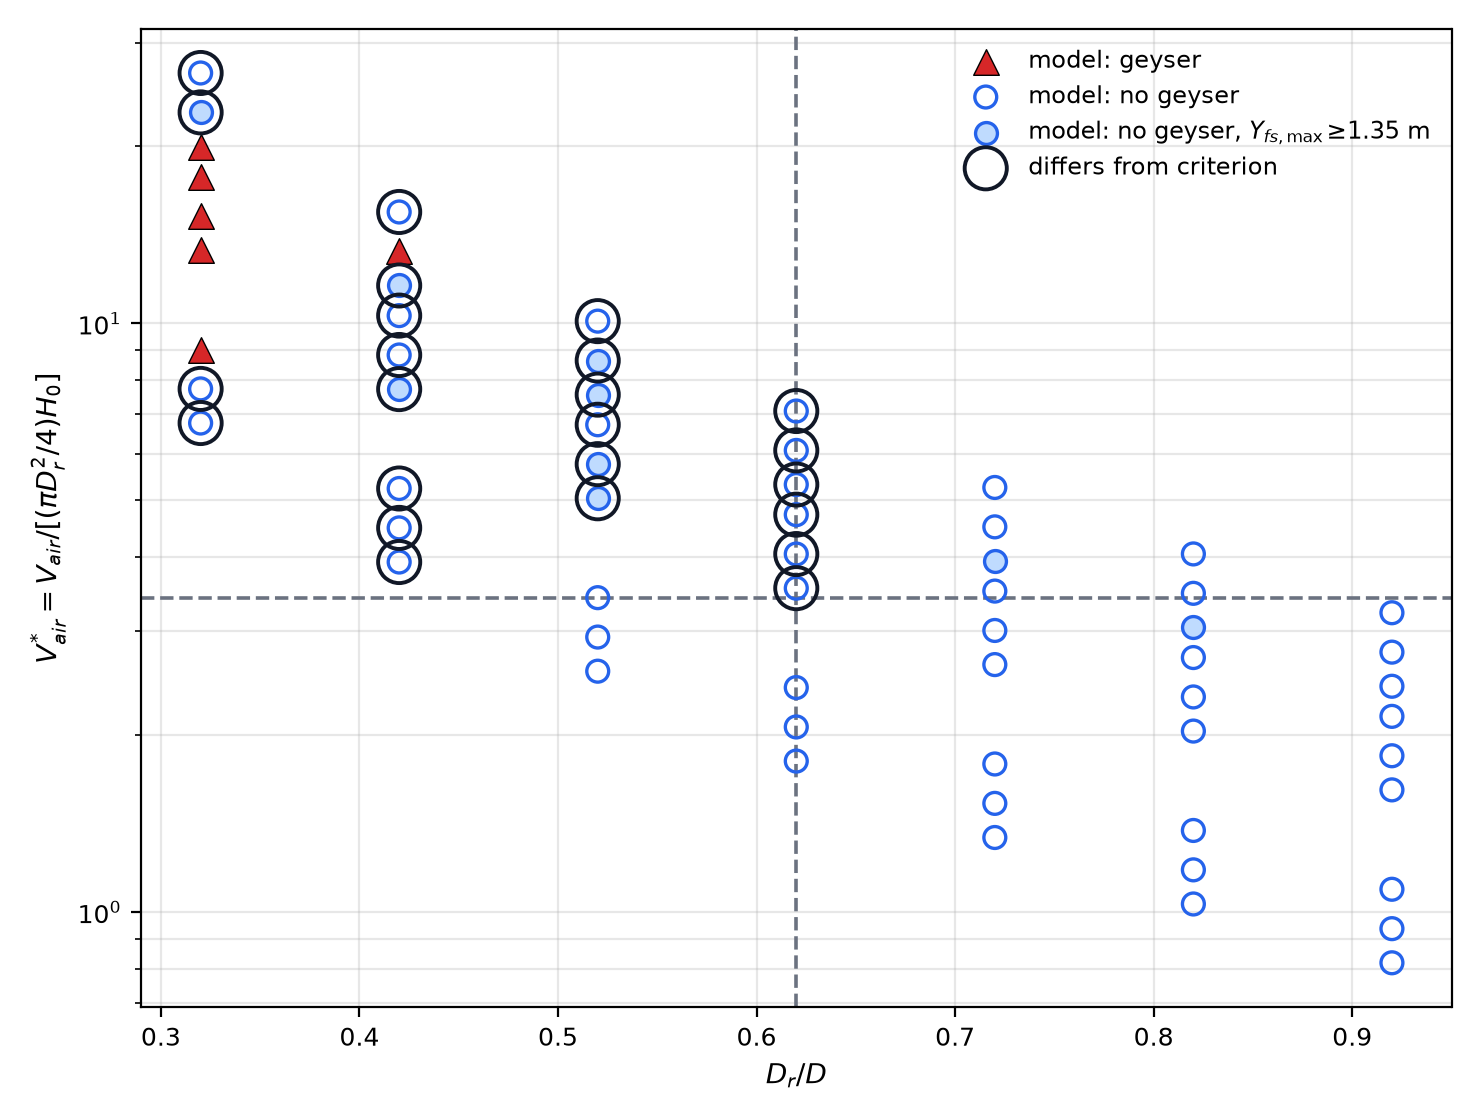
\includegraphics[width=0.85\textwidth]{cong2017_criterion_map.png}
\caption{Campaign 2 classification of 63 configurations in the criterion
plane of Eq.~(\ref{eq:cong_criterion}). Filled triangles denote model
geysering, circles non-geysering, and black rings disagreement with the
experimental criterion.}
\label{fig:cong_map}
\end{figure}

\FloatBarrier

\subsection{Campaign 3: stormwater geyser in a vertical shaft above a
junction chamber (Liu, Shao and Zhu, 2020)}
\label{sec:tests:liu2020}

The apparatus of \cite{liu2020} is a 1:20-scale model of a 27~m deep
Edmonton prototype dropshaft. A 5.80~m upstream pipe ($D=0.20$~m,
slope 1:100) feeds a transparent junction chamber
($0.30\times0.30\times0.45$~m) with an invert drop of $0.18$~m to a
5.95~m downstream pipe ($D_d=0.28$~m). A vertical shaft of diameter
$d_r=0.06$~m and height $1.22$~m is mounted at the chamber lid centre
and vents to the atmosphere. Inflow is imposed as a flow step
$Q_0\to Q_1$ with valve opening time $T_v\approx0.4$~s. Pressure
transducers PT1--PT4 monitor the shaft, the chamber lid (PT2, the
primary datum), the chamber floor, and the upstream crown
(Fig.~\ref{fig:liu_apparatus}).

\begin{figure}[htbp]
\centering
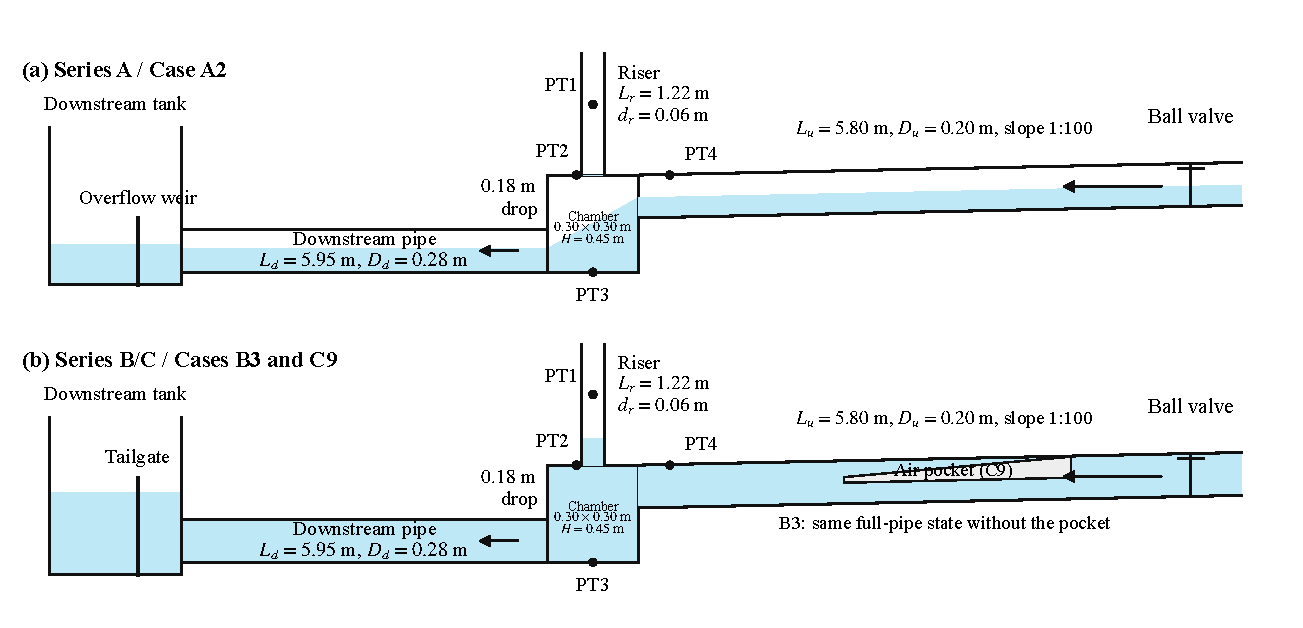
\includegraphics[width=\textwidth]{campaign3_apparatus_redrawn.pdf}
\caption{Campaign 3 apparatus and initial states, redrawn from Fig.~2 of
\cite{liu2020}.}
\label{fig:liu_apparatus}
\end{figure}

The three configurations use the documented baseline numerical settings from
the primary Campaigns~1--2 quantitative archives. The horizontal reach is a
single composite one-dimensional domain comprising the upstream pipe, chamber,
and downstream pipe. Internal momentum faces represent the chamber
connections, and a rigid-column ordinary differential equation for the shaft
water column is coupled at the lid tap. This reduced formulation does not
resolve three-dimensional chamber mixing, slug venting at the chamber gas port,
or the late-time arrival of a compressing air pocket along the upstream crown
at the level of the companion two-fluid/RTRP framework. These limitations are
stated explicitly where they affect the comparison.

\subsubsection{Branch pair A2/B3: downstream boundary flips the outcome}
\label{sec:tests:liu2020:AB}

Cases A2 and B3 share the same inflow step ($Q_0=20$, $Q_1=100$~L/s) and
differ only in the downstream tail: A2 discharges to an open channel
(weir-controlled, $h_d/D_d=1/4$), whereas B3 is initially surcharged
with a submerged tail gate. In the experiment A2 never geysered while
B3 produced a single-shoot eruption on every repetition
(Fig.~5 of \cite{liu2020}).

The unchanged model reproduces the A2/B3 branch flip. For A2, the riser column
remains below the rim ($h_{r,\max}=0.47$~m against a shaft height of
$1.22$~m). The steady chamber pressures agree with the digitized Fig.~3
record: PT3 is $5.26$~kPa against $4.99$~kPa (the model is about $5\%$ high),
and PT2 is $1.80$~kPa against $2.15$~kPa (the model is about $16\%$ low in the
standing-column head that
emerges from the composite domain rather than being prescribed). The computed
B3 run geysers, with the free surface reaching the shaft top and overflowing.
Its eruption timing is close, with peak PT2 at $1.68$~s against $1.47$~s.
However, the frozen elastic branch celerity $a_{wh}=40$~m/s underpredicts the
compressive peak amplitude: the PT2 peak is $31$~kPa against $55$~kPa
($-44\%$). A sensitivity run at $a_{wh}=80$~m/s gives $63.5$~kPa, showing that
the peak is highly sensitive to acoustic wave speed. This single sensitivity
test does not exclude a contribution from closure error. At the baseline
computed peak pressure, the experimental
regression in Fig.~7(a) gives approximately $2.50$~m
($h=0.694\,P_{\max}/\rho g+0.309$~m, $R^2=0.97$). The computed jet height is
$2.17$~m, about $0.33$~m lower.

\begin{figure}[htbp]
\centering
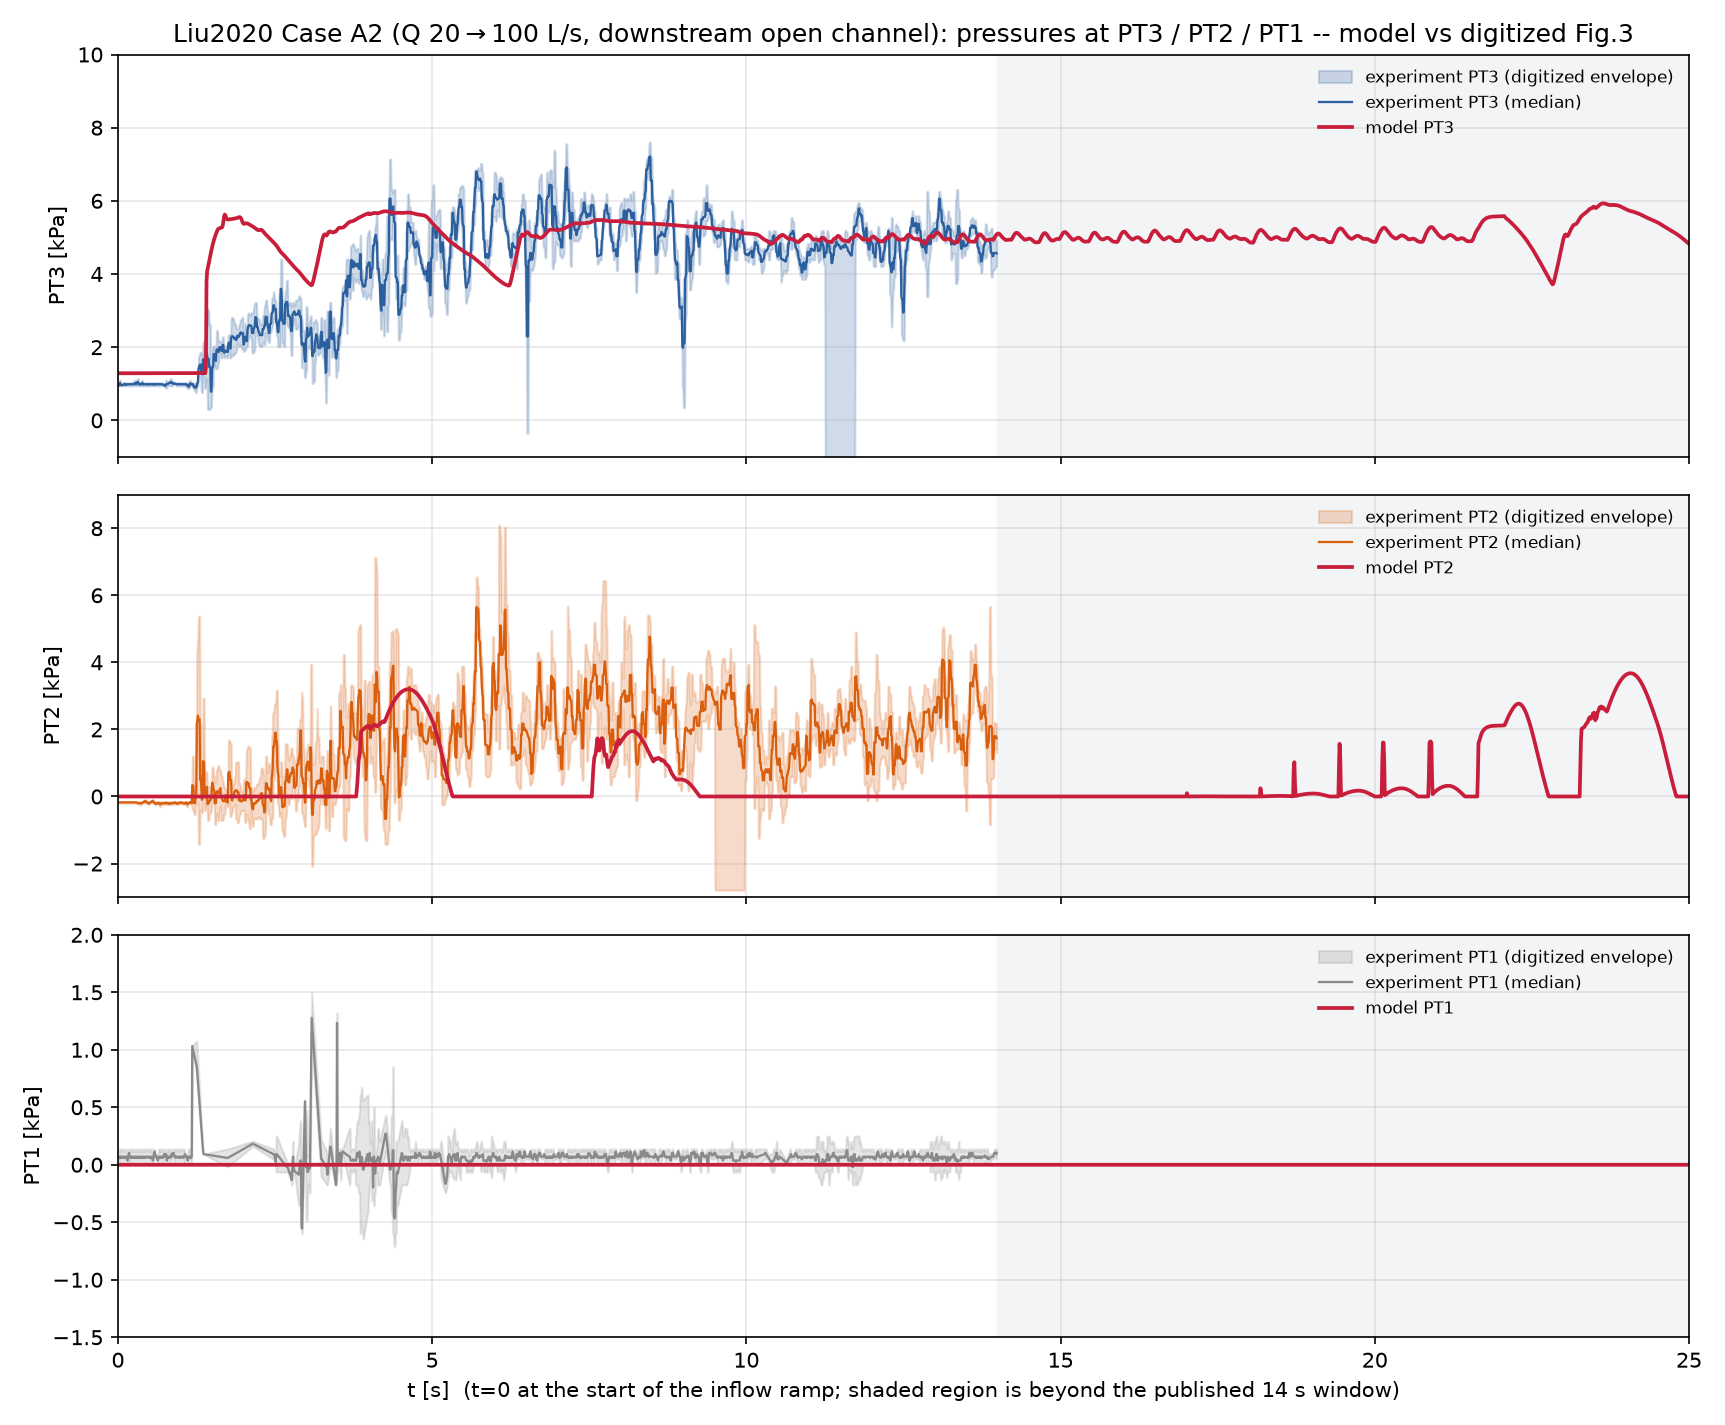
\includegraphics[width=\textwidth]{liu2020_a2_pressure.png}
\caption{Case A2 ($Q$: 20$\to$100~L/s, downstream open channel):
chamber and shaft pressures against time. Blue: digitized experimental
PT2/PT3 from Fig.~3 of \cite{liu2020}; red: present model.}
\label{fig:liu_a2_pressure}
\end{figure}

\begin{figure}[htbp]
\centering
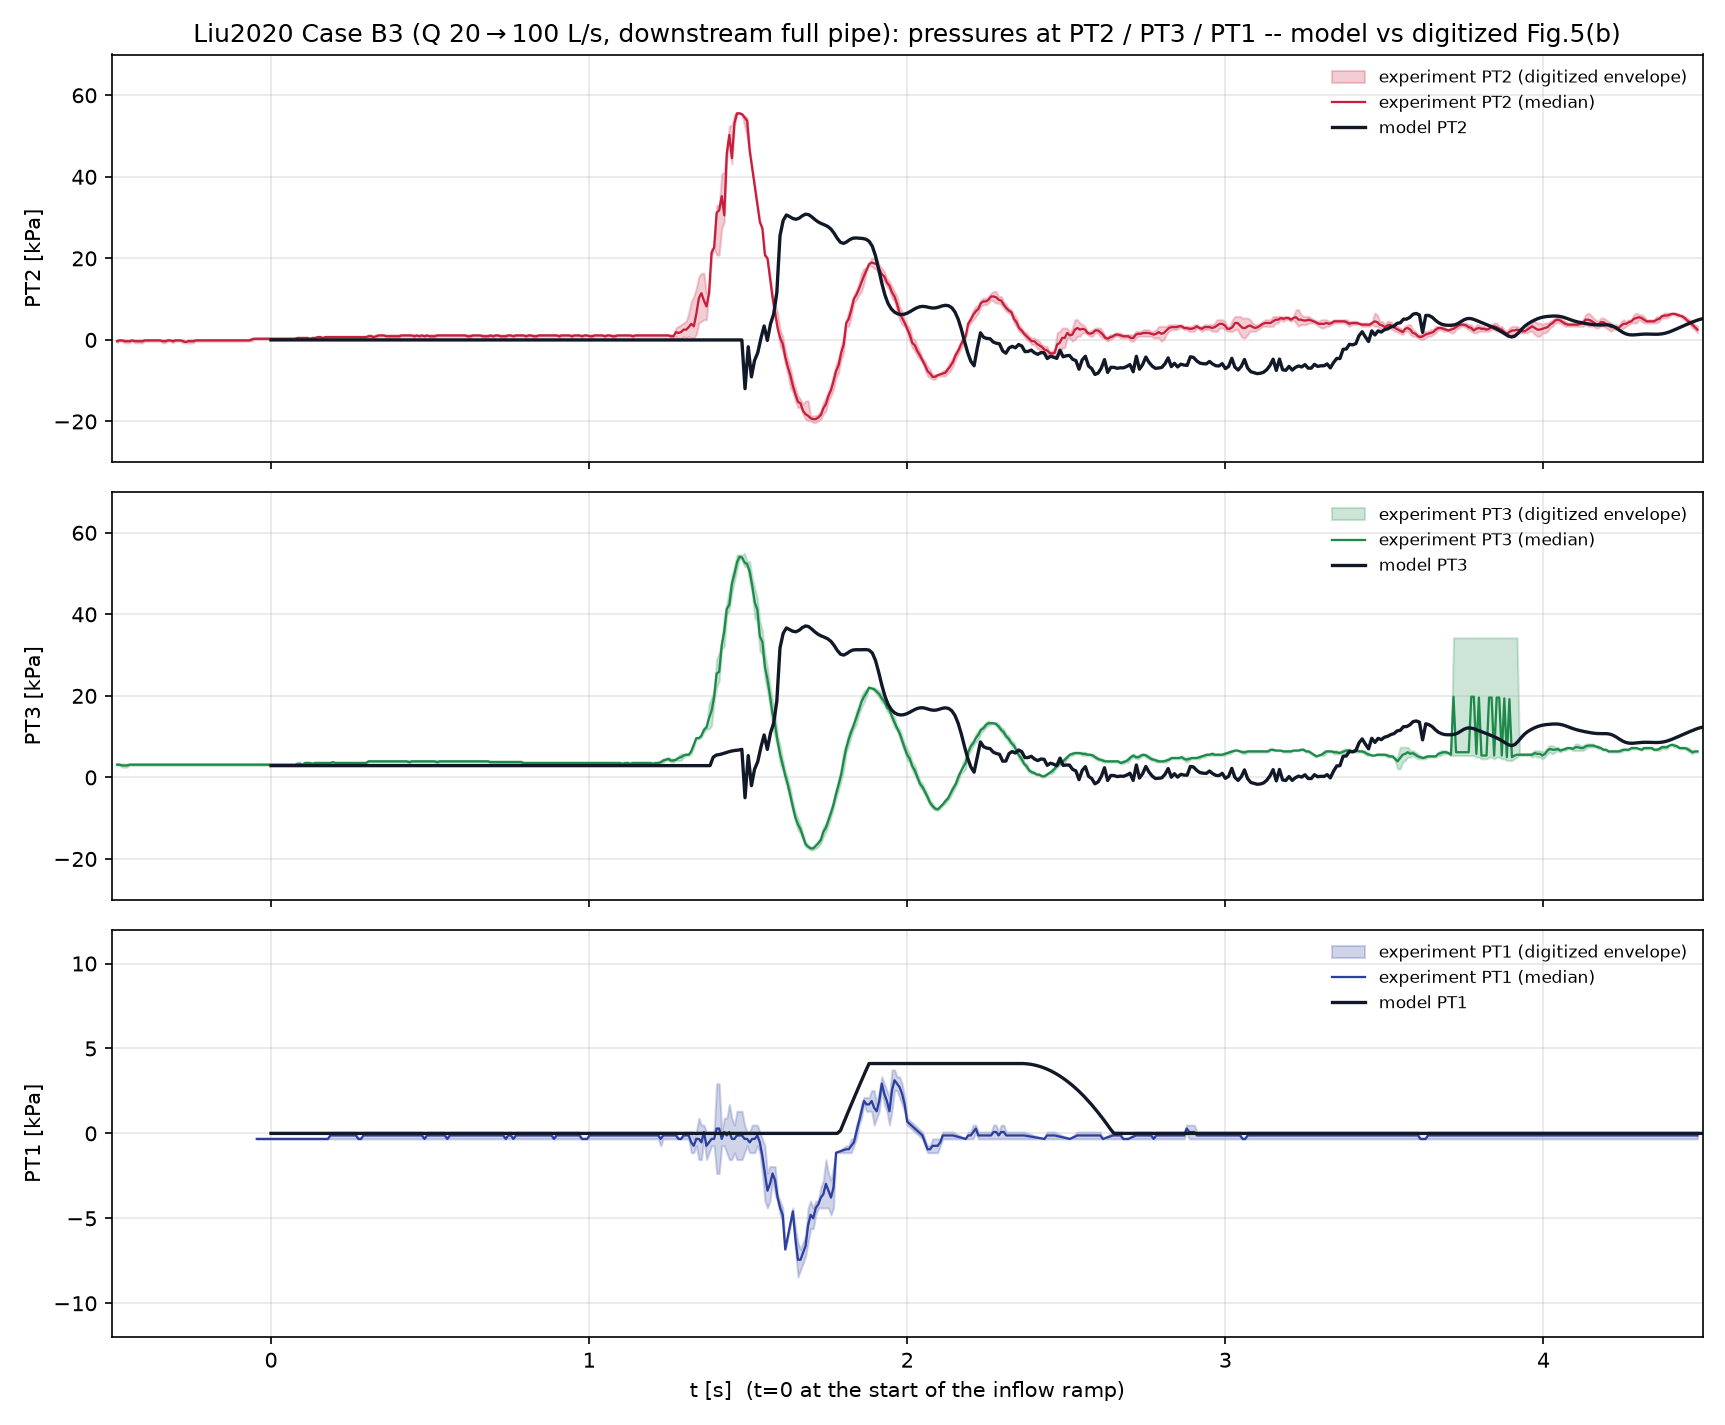
\includegraphics[width=\textwidth]{liu2020_b3_pressure.png}
\caption{Case B3 ($Q$: 20$\to$100~L/s, downstream surcharged): PT1--PT3
pressure histories. Blue: experiment \cite{liu2020}; red: present model.}
\label{fig:liu_b3_pressure}
\end{figure}

\begin{figure}[htbp]
\centering
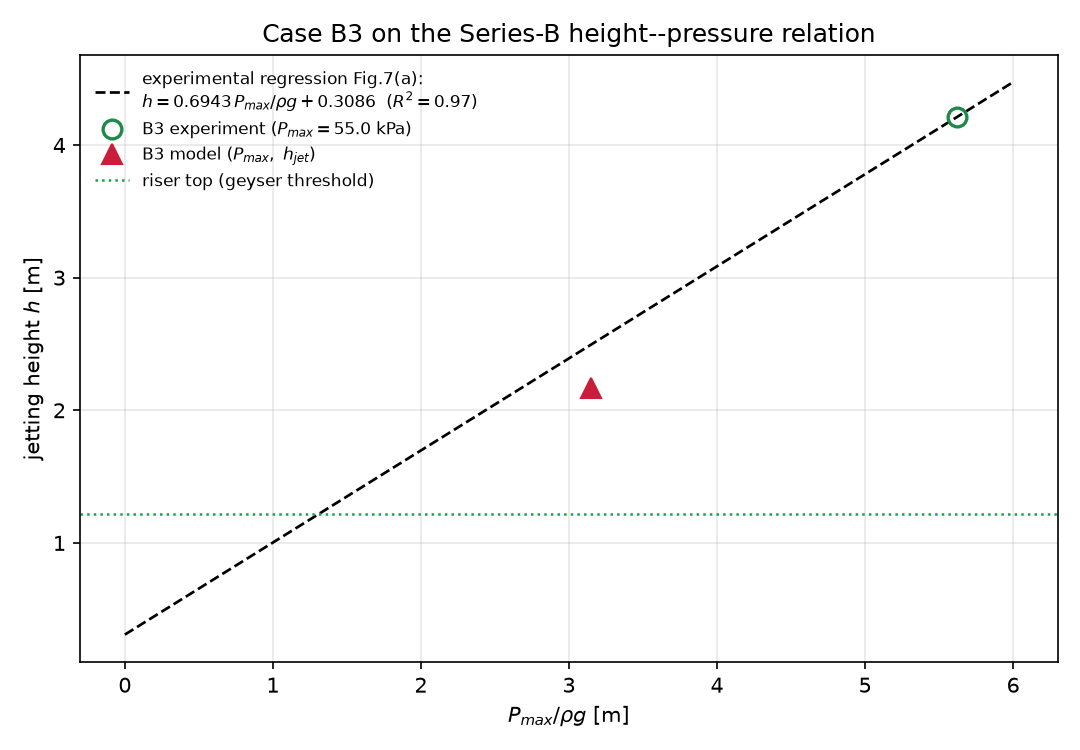
\includegraphics[width=0.72\textwidth]{liu2020_b3_h_pmax.png}
\caption{Case B3 on the eruption-height--peak-pressure diagram of
Fig.~7(a) of \cite{liu2020}. Open symbols: experimental family; filled
red circle: present model ($h=2.17$~m, $P_{\max}=31$~kPa at
$a_{wh}=40$~m/s).}
\label{fig:liu_b3_h_pmax}
\end{figure}

\subsubsection{Case C9: transient-driven geysers and the analytic
mass-oscillation model}
\label{sec:tests:liu2020:C9}

Case C9 ($Q_0=25\to Q_1=40$~L/s, surcharged downstream tail,
initial shaft column $h_{r0}=0.30$~m, sealed air wedge on the upstream
crown in the experiment) is the authors' detailed two-stage case: the
first two geysers are driven by the hydraulic transient before the
trapped pocket reaches the chamber at $t\approx6.46$~s; geysers
3--8 are pocket-driven and lie outside the present reduced solver.

For the phase-one comparison the pocket is omitted in the computation
(the all-water variant assumed in Eq.~(7) of \cite{liu2020}), while the
sealed-pocket run is retained as a qualitative cushioning check. The
analytic head at the chamber lid is
\begin{equation}
H_s(t)=h_{r0}+\frac{L_d}{gA_d}\frac{\mathrm{d}Q_u}{\mathrm{d}t}
\left(1-\cos\frac{2\pi t}{T}\right),
\qquad
T=2\pi\sqrt{\frac{L_d A_r}{gA_d}+\frac{h_{r0}}{g}},
\label{eq:liu_eq7}
\end{equation}
with $T=1.52$~s for C9.

The all-water model captures the first C9 pressure peak in both timing and
magnitude (Fig.~\ref{fig:liu_c9_phase1}). The figure compares the digitized PT2
record from Fig.~9, converted to head at the chamber-top datum, with
Eq.~(\ref{eq:liu_eq7}) and the all-water model over the first 5~s. The measured
first peak is $P_{1m}=10.69$~kPa at $t=0.50$~s, and the model gives
$11.5$~kPa at $0.54$~s. The free surface reaches the shaft top at $0.73$~s in
the experiment and $0.93$~s in the model. The oscillation period is
$T=1.45$~s in the paper (Eq.~(8)), compared with $1.13$~s in the model and
$1.52$~s in Eq.~(\ref{eq:liu_eq7}). The model period is closer to the analytic
value than to the measured period, but remains fast, consistent with the stiff
one-dimensional tail-gate coupling. After the first transient, the steady
heads agree within $\approx20\%$: the experimental PT2 final value is
$8.79$~kPa, and the model gives $10.6$~kPa. The
sealed-pocket variant qualitatively delays and cushions the first peak as in
the experiment. It then drifts after $\approx4$~s as the wedge compresses
through the reduced gas model, a phase-two process outside the stated scope.

\begin{figure}[htbp]
\centering
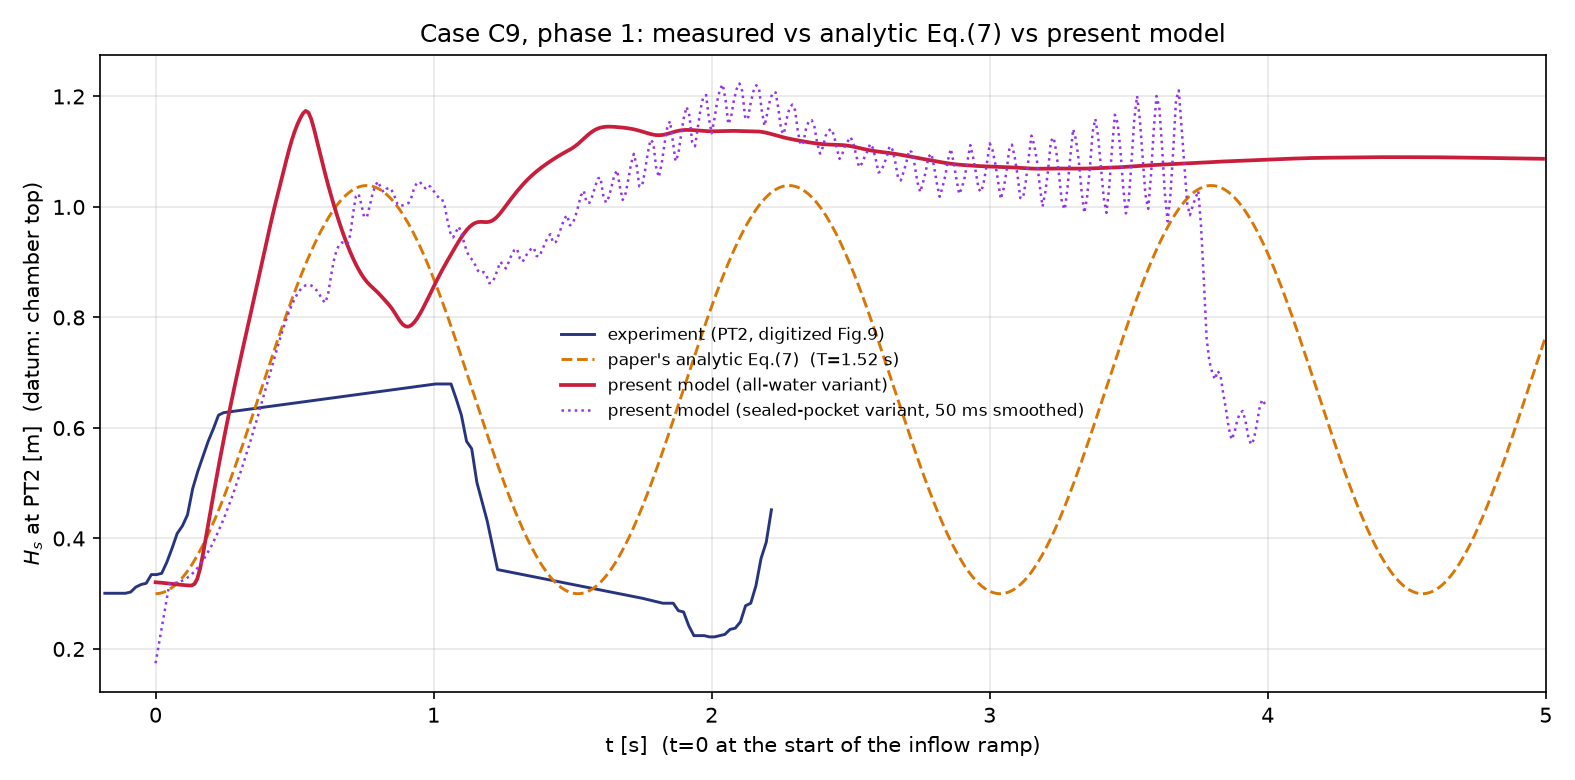
\includegraphics[width=\textwidth]{liu2020_c9_phase1.png}
\caption{Case C9, phase~1 ($t<5$~s): PT2 head $H_s$. Blue: experiment
\cite{liu2020}; orange dashed: Eq.~(\ref{eq:liu_eq7}); red: all-water model;
purple dotted: sealed-pocket variant.}
\label{fig:liu_c9_phase1}
\end{figure}

\begin{figure}[htbp]
\centering
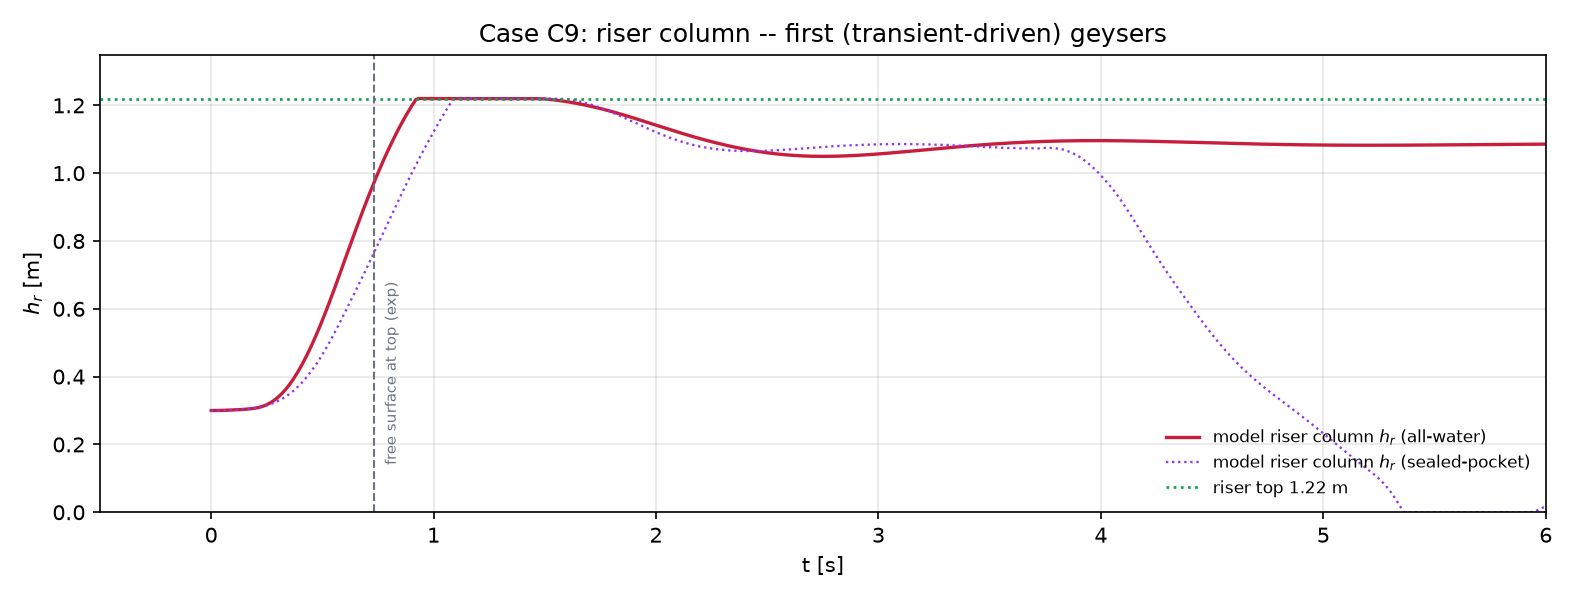
\includegraphics[width=\textwidth]{liu2020_c9_riser.png}
\caption{Case C9: shaft water-column height $h_r$ for the all-water
(solid) and sealed-pocket (dotted) variants. The dashed line marks the
experimental time at which the free surface first reaches the shaft
top in phase~1.}
\label{fig:liu_c9_riser}
\end{figure}

\begin{table}[htbp]
\centering
\caption{Campaign~3 summary metrics. Acoustic peaks use the frozen
$a_{wh}=40$~m/s; no coefficient is retuned between cases.}
\label{tab:liu_summary}
\begin{tabular}{lccc}
\toprule
Quantity & A2 (no geyser) & B3 (geyser) & C9 phase~1 \\
\midrule
Geyser? & no / no & yes / yes & yes / yes \\
PT2 steady or peak [kPa] & $1.80$ / $2.15$ & $31$ / $55$ & $11.5$ / $10.7$ \\
Peak or top-arrival time [s] & -- & $1.68$ / $1.47$ & $0.54$ / $0.50$ \\
Shaft top reached [s] & -- & $\approx1.65$ & $0.93$ / $0.73$ \\
Oscillation period [s] & $0.30$ (PT2--PT3) & -- & $1.13$ / $1.45$ \\
\bottomrule
\multicolumn{4}{l}{\footnotesize Slash-separated cells: model / experiment; single values are identified by row.}\\
\end{tabular}
\end{table}

Across the three cases, the composite-domain formulation extends the frozen
Campaign~1--2 solver to a prototype-motivated junction geometry. The A2/B3
pair reproduces the change in regime caused by the downstream boundary, and C9
phase~1 reproduces the transient mass-oscillation geyser. Agreement covers
regime selection and timing, as well as amplitude where the governing response
is hydraulic rather than acoustic. The main residuals are the
under-resolution of short compressive pressure spikes with the frozen elastic
celerity and the deliberate omission of pocket-transport physics after the
pocket reaches the chamber.

\section{Discussion}
\label{sec:discussion}

\subsection{What the framework resolves}

The comparisons in Section~\ref{sec:tests} indicate that a one-dimensional
formulation that conserves gas mass and momentum in the shaft and pipe, and
that treats trapped pockets by an equation of state on the resolved pocket
volume, is sufficient to select the geysering regime without regime-specific
inputs. In the wide-tower test the venting pathway---pocket discharge
through the tower with counter-current exchange at the mouth---sets a
pressure plateau whose level and duration are controlled by the pocket
volume and the tower hydrostatic column; both are reproduced because they
follow from conservation rather than from calibrated closures. The interface
climb velocity in the wide tower is likewise reproduced at the
Taylor-bubble scale without any drift-flux input, because the buoyant rise
of the gas core through the resolved liquid column is part of the two-fluid
solution.

The regime discrimination between Tests A and B is controlled by the tower
diameter through two competing rates that the model resolves: the rate at
which the pocket discharges gas into the tower base, and the rate at which
the tower can pass gas through its water column and vent it at the rim. In
the wide tower the column passes the gas with a modest surface rise; in the
narrow tower the same discharged volume displaces the column to the rim.
This is the mechanism identified experimentally in
\cite{vasconcelos2011}, and it emerges here from the computed state.

Campaign 2 tests whether this discrimination generalizes beyond a single
apparatus, and the answer is structured rather than uniform. Across the
63-configuration sweep of the \cite{cong2017} parameter ranges, computed
with the same frozen solver and no knowledge of the experimental
criterion, the model reproduces both end members of the regime boundary
exactly---every wide-riser configuration ($D_r/D>0.62$) and every
small-volume configuration ($V^{*}_{air}<3.42$) vents without eruption,
and the narrowest risers with large pockets erupt---and it reproduces the
interaction sense of the criterion, since both thresholds derive from the
same resolved competition: the pocket must sustain its overpressure
against the shrinking column (volume condition) faster than the riser can
vent the gas through the column (diameter condition). Inside the
transition band, however, the model is conservative: 24 of 63
configurations that the criterion marks as geysering are computed as
strong but sub-rim column lifts ($1.0$--$1.6$~m against the $1.8$-m rim),
and the corresponding two intermediate Series-B runs (B-H2, B-H3) are the
only classification misses among the seven high-speed-camera runs. All
disagreements are one-sided---no configuration erupts in the model that
the criterion excludes---so the frozen configuration errs toward missing
marginal geysers, not toward false alarms.

\subsection{Identified limitations}

The completed campaigns expose five limitations, all at the level of the
junction and closure treatment rather than of the two-fluid formulation, and
all consistent with the model simplifications listed in the companion paper
\cite{xue2026model}.

\emph{Junction base datum.} The two branches of Campaign~1 currently use
different elevation datums for the shaft-base coupling: the wide-tower run
transmits the invert piezometric head to the shaft base, while the
narrow-tower run transmits the crown pressure (the tower physically taps
the pipe crown, one bore above the invert). The crown datum is the
geometrically correct choice, and in the narrow tower the difference,
up to $\rho_l g D=0.15L$ of spurious driving head, decides between a column
pinned at the rim and the measured quasi-static stand. In the wide tower the
distinction is masked by the aerated column (the visible level includes
gas-holdup swell) and the invert coupling reproduces the measurements; a
single junction closure that carries the vertical pressure distribution
across the mouth---rather than one scalar datum---is the consolidation
target.

\emph{Narrow-shaft climb closure.} The measured interface climb in the
narrow tower ($V^{*}_{int}=1.43$, far above the Taylor-bubble scale) is
approached only when the shaft gas connected to the pocket is treated as a
pocket-fed core whose nose is raised by the mouth influx, with the influx
bounded by the Wallis counter-current flooding scale; with the dissipative
cavity celerity the computed nose speed is $0.71$---half the measured
value, but still twice the Taylor scale---because the mouth influx inherits
the reduced crown feed. These two elements
use literature constants ($C_w=0.9$) and geometric closure levels, not
per-case fits, but they are engaged only in the driven regime
($H_{a0}>Y_{fs,0}$ with gas at the junction); the undriven regime retains
the dispersed-bubble drag path. In Campaign~2's venting-without-eruption
runs the driven-path feed produces the climb in surge pulses (fastest
sustained climbs $0.7$--$1.2$~m/s) where the measurements show a steady
Taylor-scale ascent ($0.42$--$0.48$~m/s); a vertical-annular entrainment
closure conditioned on the local gas flux would unify the two paths and
smooth the pulsing.

\emph{Crown-cavity celerity and the arrival/venting trade-off.} Two
elements set the timing of the gas-phase sequence. First, a discrete bias
in the front-tracking hand-off was identified during this work and removed:
releasing the cavity nose cell at $95\%$ of the region-mean layer depth let
the detected front advance on $95\%$ of its volume budget, biasing the
transit to $1.09$ times the nominal celerity. Second, the cavity celerity
coefficient itself: Benjamin's $0.542\sqrt{gD}$ is the energy-conserving
upper bound, while real (dissipative) cavities run below it, and the
middle-pipe transits of the three experimental repetitions correspond to
$0.48$--$0.52\,\sqrt{gD}$. The frozen configuration uses the dissipative
value $0.48$ (one value for both tests), which places the arrival events
inside the repetition scatter (Test~A liftoff $7.5$ against onsets
$7.3$--$7.9$; Test~B entry $-0.13$, eruption $-0.20$). The trade-off is
stated openly: the same crown current that carries the cavity nose also
feeds the vent and the narrow-tower pocket-fed core, so the reduced
celerity delays the venting-stage events (head-decay onset and interface
breakthrough late by $0.4$--$0.6$ units in both tests) and halves the
computed narrow-tower climb rate ($V^{*}_{int}=0.71$ against $1.43$). A
closure that separates the nose celerity from the vent feed rate---the
former set by the front dynamics, the latter by the pocket overpressure---%
is the identified refinement.

\emph{Film-flow pocket topology in the venting branch.} In the wide-tower
experiment the gas ascends the shaft as a single Taylor pocket that remains
pneumatically continuous with the pipe pocket: its wall film is
shear-supported, so the pocket pressure follows the weight of the water
column standing \emph{above the pocket nose}, the transducer head decays
gradually \emph{during} the climb, and the free surface creeps upward by
pocket expansion (Figs.~5 and~10 of \cite{vasconcelos2011}; their TPA model
encodes this topology by construction, as a lumped pocket with a
Batchelor-type film-flow closure). In the present field formulation the
tower gas transits as a dispersed phase interleaved with liquid, the tower
base carries the weight of the full standing column, and the computed head
therefore holds its plateau until breakthrough
(Fig.~\ref{fig:caseA_tpa}); the climb-phase free-surface creep is likewise
absent ($V^{*}_{fs}\approx0$ against the measured $0.048$). We tested a
connected-pocket closure that relaxes the pipe-pocket pressure toward the
hydrostatic environment of the tower gas nose while crediting the
transferred volume to the tower (retained as a solver option). It
reproduces the free-surface creep quantitatively ($Y^{*}_{fs}$ from $0.59$
to $0.64$ during the climb, against $0.55$--$0.65$ measured) without
degrading the validated event times, but the head history develops a
spurious hump near the catch instead of the measured monotone decay, and
more aggressive relaxation destabilizes the junction dynamics. We conclude
that the during-climb head decay is a property of the coherent-pocket
topology that a dispersed one-dimensional two-fluid closure cannot
represent stably at this grid scale---consistent with
\cite{vasconcelos2011}'s own choice of a lumped-pocket formulation for
exactly this regime---and the frozen configuration retains the
plateau-then-collapse behaviour, which preserves the plateau level, the
collapse onset time, and the interface kinematics.

\emph{Release oscillation damping.} The underdamped release-piston
oscillation visible in both tests is a genuine mode of the system---a water
column on a gas spring---and is annotated as such in the experimental
schematic of \cite{vasconcelos2011}; the experimental traces damp within
about one time unit, the model within several. The damping in the
experiment is provided by three-dimensional mixing losses at the valve and
coupling, which the constant valve and junction loss coefficients capture
in the mean but not cycle-resolved. In the narrow tower the surviving
oscillation also lets the column splash briefly to the rim during the
release swing before it settles at the quasi-static stand; in Campaign~2
the same simplification sharpens the B-H1 eruption jet ($1.71$ against
$0.92$~m/s as event speeds).

\emph{Volume-neutral mouth exchange in the reservoir-fed layout.} The
inverted-glug exchange at the tee mouth---gas up, an equal water volume
down---is what keeps the pocket pressure intact while gas transits a
standing column, and it is essential to the B-H1 geyser: without it the
narrow-riser pocket cannot rebuild the overpressure whose release ejects
the column. But in the reservoir-fed layout of Campaign~2 the same
exchange cancels part of the one-to-one column lift that the entering gas
volume should produce, and the cancellation grows with riser width: the
computed B-H6 free-surface rise is $+0.12$~m against the measured
$+0.63$~m, and across the 63-configuration sweep the under-lift accounts
for the one-sided transition-band misses (Section~\ref{sec:tests:cong2017:map}).
Gating the exchange off for reservoir-backed cases was tested and
rejected: it restores the wide-riser lift but opens the narrow pocket's
volume during the balanced venting phase, its pressure never rebuilds, and
the B-H1 geyser is lost. The two branches place conflicting demands on a
single mouth closure; a formulation that meters the exchange by the local
counter-current capacity of the mouth (rather than volume neutrality) is
the identified refinement, together with the entrainment closure above.

\subsection{Scope of the present validation}

The completed campaigns cover three apparatuses and three kinds of
evidence: time-resolved two-regime histories in a single-shaft geometry
(Campaign~1), regime classification over a systematic parameter sweep in
a riser--constant-head geometry (Campaign~2), and a prototype-motivated
junction-chamber geometry with a downstream-boundary branch pair and a
transient mass-oscillation geyser (Campaign~3), all under one frozen solver
configuration and a fully synchronous junction coupling. Within this scope
the conclusions are: in Campaign~1, regime selection is exact and both
branches are quantitative in their pressure and interface histories, with
absolute event times uniformly early by $0.5$--$0.7$ time units; in
Campaign~2, the regime boundary is reproduced in structure (both end
members, the interaction sense, the branch differentiation of the pipe-end
pressure) with a one-sided conservative bias in the transition band (5/7
of Series~B, 39/63 of the sweep, no false positives); in Campaign~3,
the A2/B3 pair flips branch with downstream boundary alone, C9 phase~1
matches the first transient geyser in timing and first-peak amplitude
against both measurement and Eq.~(\ref{eq:liu_eq7}), while compressive
spikes and pocket-driven late geysers remain limited by the frozen
elastic celerity and the reduced one-dimensional chamber treatment.
Three caveats bound the claims. First, the narrow-shaft closure elements of Test~B
(crown-datum base coupling, pocket-fed core, flooding-limited entry) are
engaged only in the driven regime; their consolidation with the wide-tower
configuration into a single junction closure is pending. Second, the
volume-neutral mouth exchange places conflicting demands on the two
Campaign-2 branches (see above), and its resolution will move the
transition-band classifications. Third, Campaign~3 uses a composite
one-dimensional chamber representation and does not resolve pocket
transport to the junction or chamber gas venting; comparison at larger
scale \cite{muller2017} remains a separate target.

\section{Conclusions}
\label{sec:conclusions}

This paper applied the decoupled two-fluid cut-cell finite-volume framework
of \cite{xue2026model} to laboratory geysering experiments, representing the
vertical shaft as the same one-dimensional two-fluid system rotated to the
vertical and coupled to the horizontal conduit through junction-loss
closures. Three campaigns were completed, all computed from the experimental
initial conditions without prescribed release rates or per-case fitting.

Against the ventilation-shaft experiments of Vasconcelos and Wright
\cite{vasconcelos2011}, the model selected the correct regime in both the
non-geysering and geysering configurations. In the non-geysering branch it
reproduced the pressure plateau level and duration, the onset of the
terminal venting decay, the maximum free-surface rise, and the air--water
interface climb velocity. In the geysering branch it reproduced the
pre-eruption quasi-static stand of the tower column ($0.84L$ against
$0.82L$), the crown-datum pressure plateau ($0.76$ against $0.76$), the
eruption to the shaft rim observed in every repetition, the interface and
free-surface climb velocities ($V^{*}_{int}=1.19$ against $1.43$;
$V^{*}_{fs}=0.42$ against $0.44$), and the sharp plateau--collapse of the
head at pocket venting; the narrow-shaft closure combines a crown-datum
base coupling, a pocket-fed gas core, and a Wallis flooding limit on the
entry flux, using geometric and literature-scale constants. The remaining
biases are a uniform early shift of the gas-phase event times
($0.3$--$0.6$ time units, within the uncertainty of the hand-operated
valve opening) and an underdamped release oscillation.

Against the horizontal-pipe/vertical-riser experiments of Cong, Chan and
Lee \cite{cong2017}, computed with the same frozen solver under the fully
synchronous coupling, the model reproduced the branch structure of the
published two-parameter geysering criterion: the geysering end member
(B-H1, with its compression-surge drive to $1.71\,H_0$), the entire
no-geysering half-plane $D_r/D>0.62$ and small-volume region, and the
branch differentiation of the pipe-end pressure that only a coupled
riser--pipe computation can produce. Its errors are one-sided and
conservative: two intermediate Series-B runs and 24 of 63 sweep
configurations that geyser in the experiment are computed as strong but
sub-rim column lifts, with no false positives; the bias is traced to the
volume-neutral mouth exchange, whose conflicting demands in the two
branches are documented as the primary closure target.

Against the junction-chamber experiments of Liu, Shao and Zhu
\cite{liu2020}, computed with the same frozen solver in a composite
one-dimensional representation, the model reproduced the downstream-boundary
branch flip between Cases A2 and B3, placed the B3 eruption on the
experimental $h$--$P_{\max}$ regression line (with acoustically
under-resolved peaks at $a_{wh}=40$~m/s), and matched the first transient
geyser of Case C9 in peak timing and magnitude against both measurement
and the authors' Eq.~(\ref{eq:liu_eq7}). Pocket-driven geysers after
pocket arrival at the chamber were declared out of scope.

These results support the use of gas-conserving one-dimensional two-fluid
models for system-scale geysering screening, where the primary question is
regime selection and venting behaviour rather than jet detail, and they
identify the junction and entrainment closures as the targets for
quantitative improvement in the geysering branch.


\section*{Data Availability Statement}

The data and materials supporting the findings of this study are available
from the corresponding author upon reasonable request. A persistent archive
identifier will be added if the project repository is deposited before
submission.

\section*{Declaration of Generative AI Use}

Generative AI tools were used to assist language revision and manuscript
organization. The authors critically reviewed and edited all generated
material and take full responsibility for the content of the manuscript.

\bibliographystyle{elsarticle-num}
\bibliography{references}

\end{document}
